\section{Evaluation}
\label{sec:eval}

The GPU measurements share one node and one engine, and they differ by model, tensor-parallel width, and workload.
\S\ref{sec:eval-gpu} is the full GSM8K forest on Qwen3-14B at $\mathrm{tp}{=}2$.
\S\ref{sec:eval-app} is a control-plane cost model of \app, with no GPU, against APC, hash prefill, baseline prefill--decode disaggregation, \sys, and three decoding-time pruners.
\S\ref{sec:eval-plus} runs ForkServe+ on Qwen3-8B at $\mathrm{tp}{=}2$ and $\mathrm{tp}{=}4$.
\S\ref{sec:eval-mt} is a three-turn Tree-of-Thoughts on Qwen3-4B and Qwen3-8B, one problem per generate.
\S\ref{sec:eval-multi} repeats the forest on six families at $n{=}40$.
\S\ref{sec:eval-sens} sweeps branching, depth, pruning, and batch width on Llama-3-8B, Mistral-7B, and DeepSeek-R1-Distill-Llama-8B, then runs a $2048$-token contest forest on that DeepSeek model and on Qwen3-4B.

\paragraph{Setup.}
GPU runs use vLLM on four A100-SXM4 40GB GPUs, with \texttt{bfloat16} weights and $\mathrm{tp}{=}2$ or $4$.
The models are Qwen3-14B, Qwen3-8B, Qwen3-4B, Qwen2.5-Math-1.5B, Llama-3-8B, Mistral-7B, and DeepSeek-R1-Distill-Llama-8B.
Tree-of-Thoughts uses $k{=}4$ and a $512$-token budget ($2048$ on the contest forest), in batches of eight.
The three-turn run in \S\ref{sec:eval-mt} issues one problem per generate.
A math answer is correct when its final number matches the reference.

\subsection{GPU forest}
\label{sec:eval-gpu}

\paragraph{Setup.}
This section uses Qwen3-14B at $\mathrm{tp}{=}2$.
The GSM8K test set has $1319$ problems.
Each problem is expanded with four thoughts and decoded for at most $512$ tokens, in $165$ batches of eight.
Accuracy is the fraction of problems whose final number matches the reference.

\begin{table}[t]
\centering
\caption{GSM8K test, Qwen3-14B, $\mathrm{tp}{=}2$, $n{=}1319$.
Median over $165$ batches of eight.
Best storage in green.}
\label{tab:gsm}
\scriptsize
\setlength{\tabcolsep}{3.5pt}
\setlength{\aboverulesep}{0.4pt}
\setlength{\belowrulesep}{0.4pt}
\begin{tabular}{lrrr}
\rowcolor{tblhead}
\toprule
 & recompute & APC & FS \\
\midrule
Accuracy & $0.847$ & $0.844$ & $0.845$ \\
\rowcolor{tblalt}
Peak KV, median (tok) & $4136$ & $1430$ & \win{$1030$} \\
Peak KV, max (tok) & $4944$ & $1632$ & \win{$1232$} \\
\rowcolor{tblalt}
Peak / APC & $2.89\times$ & $1.00\times$ & \win{$0.72\times$} \\
Fan-out, median (ms) & $326$ & $87$ & $140$ \\
\rowcolor{tblalt}
Generation (min) & --- & $18.6$ & $18.9$ \\
KV saving vs.\ rec. & --- & $0.65$ & \win{$0.75$} \\
\bottomrule
\end{tabular}
\end{table}

\paragraph{Storage and expand latency.}
\Cref{tab:gsm} reports the storage result and the expand-latency gap that \app is designed to close.
Median peak KV is $0.72\times$ APC and $0.25\times$ recompute, and accuracy stays within one point of both.
Storage and fan-out do not share that ordering: median fan-out is $140$\,ms for \sys and $87$\,ms for APC, because copy-on-write and abort execute on the expand path, whereas an APC hash hit does not.
End-to-end generation remains within $2\%$ of APC ($18.9$ vs.\ $18.6$ minutes).
The same peak ordering, $0.58$--$0.80\times$ APC, holds on seven math sets for Qwen3-14B, Qwen3-8B, and DeepSeek-R1-Distill-Llama-8B at $\mathrm{tp}{=}2$ and $\mathrm{tp}{=}4$.
The peak is unchanged when the tensor width doubles; it follows the committed path, as \eqref{eq:mem} requires.

\subsection{Prefill pruning}
\label{sec:eval-app}

\paragraph{Setup.}
Control plane, no GPU.
Ten sessions, $k{=}4$, $L{=}256$, $\ell{=}32$.
Two of four residuals fail the draft score; the winner is index $0$.
Prefill time is $\ell\times 12\,\mu\mathrm{s}/\mathrm{token}$; P/D transfer is $2\,\mu\mathrm{s}/\mathrm{token}$.
APC and hash prefill publish blocks only after a request materializes them, so the first fan-out clones $k$ trunks.
Baseline disaggregation uses that prefill and then transfers the live token span.
\sys aliases the trunk by pointer swap and prefills the $k$ residuals.
\app adds hash skip, draft prune, early abort, lazy abort, and a connector that inserts only retained residuals.

\begin{table}[t]
\centering
\caption{Control-plane fan-out ($10$ sessions, $k{=}4$, $L{=}256$, $\ell{=}32$).
Bottleneck in red; ForkServe+ in green.
Not GPU wall-clock.}
\label{tab:app}
\scriptsize
\setlength{\tabcolsep}{2.2pt}
\setlength{\aboverulesep}{0.35pt}
\setlength{\belowrulesep}{0.35pt}
\begin{tabular}{llrrrrrr}
\rowcolor{tblhead}
\toprule
Phase & Method & $W$ & $T_{\mathrm{fan}}$ & $X$ & peak & skip & prune \\
\midrule
\multirow{5}{*}{fan-out}
 & APC & \botn{$11520$} & $139.0$ & $0$ & $11520$ & $0$ & $0$ \\
\rowcolor{tblalt}
 & hash & \botn{$11520$} & $139.0$ & $0$ & $11520$ & $0$ & $0$ \\
 & P/D disagg. & \botn{$11520$} & \botn{$162.1$} & \botn{$11520$} & $11520$ & $0$ & $0$ \\
\rowcolor{tblalt}
 & FS & $3840$ & $47.1$ & $0$ & $3840$ & $0$ & $0$ \\
 & ForkServe+ & \win{$2592$} & \win{$31.4$} & \win{$32$} & \win{$2880$} & $9$ & $30$ \\
\midrule
 & ForkServe+ / APC & \win{$-77.5\%$} & \win{$-77.4\%$} & --- & \win{$-75\%$} & --- & --- \\
\bottomrule
\end{tabular}
\end{table}

\paragraph{Fan-out.}
\Cref{tab:app} is the comparison the GPU gap motivates.
% and \Cref{fig:eval-stack} shows occupancy over the expand--abort--decode phase.
On the first expand, hash prefill matches APC: the blocks are unpublished, so the hash probe does not remove the cloned trunks.
Baseline disaggregation exceeds APC ($162$ vs.\ $139$\,ms) because it transfers that clone.
\sys removes the clone by aliasing the trunk ($3840$ prefill tokens, $47$\,ms).
\app then withholds prefill from $30$ of the $40$ residuals, which reduces $T_{\mathrm{fan}}$ to $31.4$\,ms and the connector payload from $11520$ tokens to $32$.

\paragraph{Decoding-time pruning.}
\Cref{tab:decode-prune} runs ESC~\cite{esc}, Speculative Rejection~\cite{specrej}, and DPTS~\cite{dpts} on this same fan-out.
Each method prefills the shared trunk once.
The length of the decode that produces the prune score is the length published for that method.
ESC stops after a window of $5$ agreeing samples; this fan-out has four children and two low-score answers, so the window stays open and every child is decoded to the $512$-token budget.
Speculative Rejection is charged its partial-reward horizon $\tau{=}256$ and then drops the lower half ($\alpha{=}0.5$); the memory-limit trigger in that paper would not fire at $k{=}4$, so $\tau$ is the earlier checkpoint.
DPTS early-stops after its $100$-token mini-step.
The two low-score children are the ones removed, and the winner is kept.
Decoded tokens use the same $12\,\mu\mathrm{s}/\mathrm{token}$ clock.
DPTS is the earliest cut of the three and still decodes $4000$ tokens before the drop, $2000$ of them on losers, reaching the cut at $78.7$\,ms.
\app has already withheld those residuals: $0$ tokens on losers and $T_{\mathrm{fan}}{=}31.4$\,ms.

\begin{table}[t]
\centering
\caption{Decoding-time pruning on the \Cref{tab:app} fan-out ($10{\times}4$, $L{=}256$).
Decode-to-cut is the prefix that must be generated before a child can be dropped.
``On losers'' counts that prefix on the two low-score children.
Same $12\,\mu\mathrm{s}/\mathrm{token}$ clock. Not GPU wall-clock.}
\label{tab:decode-prune}
\scriptsize
\setlength{\tabcolsep}{3.2pt}
\setlength{\aboverulesep}{0.4pt}
\setlength{\belowrulesep}{0.4pt}
\begin{tabular}{lrrrrr}
\rowcolor{tblhead}
\toprule
 & prefill & decode & on losers & peak & $T_{\mathrm{cut}}$ \\
\midrule
ESC & $2560$ & \botn{$20480$} & \botn{$10240$} & \botn{$23040$} & \botn{$276.5$} \\
\rowcolor{tblalt}
Spec.\ Rejection & $2560$ & $10240$ & $5120$ & $12800$ & $153.6$ \\
DPTS & $2560$ & $4000$ & $2000$ & $6560$ & $78.7$ \\
\rowcolor{tblalt}
ForkServe+ & $2592$ & \win{$0$} & \win{$0$} & \win{$2880$} & \win{$31.4$} \\
\bottomrule
\end{tabular}
\end{table}

% Temporarily omitted from the paper (Figure 4, stacked KV occupancy).
\iffalse
\begin{figure*}[t]
\centering
\resizebox{\textwidth}{!}{\begin{tikzpicture}[
  font=\scriptsize\sffamily,
  >=Latex,
]
\definecolor{Tr}{HTML}{7EB6D9}
\definecolor{Rs}{HTML}{F4A582}
\definecolor{Sp}{HTML}{66C2A5}
\definecolor{Cl}{HTML}{B3B3B3}

% Stacked occupancy over a batch. y-scale in tokens (GPU medians / control-plane shape).
% Time: 0 open, 20 fork, 40 prefill, 60 abort, 80--100 decode.
% (a) three systems on GSM8K 14B (measured peak: rec 4136, APC 1430, FS 1030).
% (b) two workloads at n=40 (GSM8K APC 1512 / FS 1112; Game24 APC 1287 / FS 791).

% ---- helper: one stacked panel ----
% We inline 6 panels.

% ===== (a) =====
\node[font=\scriptsize\bfseries, anchor=west] at (0,5.55) {(a) Three systems, GSM8K $n{=}1319$ (one batch of eight)};

% Per-panel y-scale so each stack fills (reference style). Peak is in the title.
% -- Recompute, max 4.2k → 2.00cm --
\begin{scope}[shift={(0,2.85)}]
  \foreach \y/\lab in {0/0, 2.1/2k, 4.2/4k} {
    \draw[black!12] (0,\y*0.476) -- (4.55,\y*0.476);
    \node[font=\tiny, text=black!50, anchor=east] at (-0.08,\y*0.476) {\lab};
  }
  \fill[Cl] (0.15,0) -- (1.00,1.48) -- (1.90,1.55) -- (4.40,1.55) -- (4.40,0) -- cycle;
  \fill[Rs] (1.00,1.48) -- (1.90,1.98) -- (4.40,1.98) -- (4.40,1.55) -- (1.90,1.55) -- cycle;
  \node[font=\tiny] at (2.80,0.78) {$79.2\%$};
  \node[font=\tiny, text=fsorange!80!black] at (2.80,1.76) {$20.8\%$};
  \foreach \x/\lab in {0.15/0, 1.90/40, 4.40/100} {
    \node[font=\tiny, text=black!50] at (\x,-0.22) {\lab};
  }
  \node[font=\tiny, anchor=south] at (2.25,2.10) {Recompute \quad peak $4136$};
\end{scope}

% -- APC, max 1.50k → 2.00cm --
\begin{scope}[shift={(5.05,2.85)}]
  \foreach \y/\lab in {0/0, 0.75/0.8k, 1.50/1.5k} {
    \draw[black!12] (0,\y*1.333) -- (4.55,\y*1.333);
    \node[font=\tiny, text=black!50, anchor=east] at (-0.08,\y*1.333) {\lab};
  }
  \fill[Tr] (0.15,0) -- (1.00,1.25) -- (1.90,1.37) -- (4.40,1.37) -- (4.40,0) -- cycle;
  \fill[Rs] (1.00,1.25) -- (1.90,1.90) -- (4.40,1.90) -- (4.40,1.37) -- (1.90,1.37) -- cycle;
  \node[font=\tiny] at (2.80,0.68) {$68.4\%$};
  \node[font=\tiny, text=fsorange!80!black] at (2.80,1.64) {$31.6\%$};
  \foreach \x/\lab in {0.15/0, 1.90/40, 4.40/100} {
    \node[font=\tiny, text=black!50] at (\x,-0.22) {\lab};
  }
  \node[font=\tiny, anchor=south] at (2.25,2.10) {APC \quad peak $1430$};
\end{scope}

% -- FS, max 1.10k → 2.00cm --
\begin{scope}[shift={(10.10,2.85)}]
  \foreach \y/\lab in {0/0, 0.55/0.6k, 1.10/1.1k} {
    \draw[black!12] (0,\y*1.818) -- (4.55,\y*1.818);
    \node[font=\tiny, text=black!50, anchor=east] at (-0.08,\y*1.818) {\lab};
  }
  \fill[Tr] (0.15,0) -- (1.00,1.55) -- (1.90,1.55) -- (2.55,1.55) -- (4.40,1.70) -- (4.40,0) -- cycle;
  \fill[Rs] (1.00,1.55) -- (1.90,1.95) -- (2.55,1.95) -- (2.55,1.55) -- cycle;
  \fill[Sp] (2.55,1.55) -- (4.40,1.87) -- (4.40,1.70) -- cycle;
  \node[font=\tiny] at (1.70,0.78) {$88.1\%$};
  \node[font=\tiny, text=fsorange!80!black] at (2.15,1.76) {$11.9\%$};
  \foreach \x/\lab in {0.15/0, 1.90/40, 4.40/100} {
    \node[font=\tiny, text=black!50] at (\x,-0.22) {\lab};
  }
  \node[font=\tiny, anchor=south] at (2.25,2.10) {\sys{} \quad peak $1030$};
\end{scope}

% ===== (b) =====
\node[font=\scriptsize\bfseries, anchor=west] at (0,2.35) {(b) Two workloads, $n{=}40$ (GSM8K vs.\ Game24)};

% GSM8K APC vs FS stacked as two systems in one panel? Reference has 3 schedulers.
% Three panels: APC / FS / FS+ for GSM8K (left cluster) is too many.
% Do: GSM8K (APC+FS overlay stacked) | Game24 (APC+FS) | mix percentages
% Cleaner: three panels APC, FS, FS+ but only two workloads as two stacked hues? 
% Match reference: 3 panels = APC, FS, APP; each stacks GSM8K (bottom) + Game24 (top) as two "models"

\begin{scope}[shift={(0,0)}]
  \foreach \y in {0,0.8,1.6} {
    \draw[black!12] (0,\y*0.95) -- (4.55,\y*0.95);
    \node[font=\tiny, text=black!50, anchor=east] at (-0.08,\y*0.95) {\y k};
  }
  % APC: GSM8K 1.51 + Game24 1.29 as stacked share of a 2-workload mix
  % Show occupancy of GSM8K (bottom teal) and Game24 (top orange) under APC
  \fill[Tr] (0.15,0) -- (1.20,0.68) -- (2.20,0.72) -- (4.40,0.72) -- (4.40,0) -- cycle;
  \fill[Rs] (0.15,0) -- (1.20,0.68) -- (2.20,1.34) -- (4.40,1.34) -- (4.40,0.72) -- (2.20,0.72) -- (1.20,0.68) -- cycle;
  \node[font=\tiny] at (3.10,0.36) {$54.0\%$};
  \node[font=\tiny, text=fsorange!80!black] at (3.10,1.02) {$46.0\%$};
  \foreach \x/\lab in {0.15/0, 2.20/50, 4.40/100} {
    \node[font=\tiny, text=black!50] at (\x,-0.20) {\lab};
  }
  \node[font=\tiny, anchor=south] at (2.25,1.68) {APC \quad $1512{+}1287$};
\end{scope}

\begin{scope}[shift={(5.05,0)}]
  \foreach \y in {0,0.8,1.6} {
    \draw[black!12] (0,\y*0.95) -- (4.55,\y*0.95);
  }
  \fill[Tr] (0.15,0) -- (1.20,0.50) -- (2.20,0.53) -- (4.40,0.53) -- (4.40,0) -- cycle;
  \fill[Sp] (1.20,0.50) -- (2.20,0.91) -- (4.40,0.91) -- (4.40,0.53) -- (2.20,0.53) -- cycle;
  \node[font=\tiny] at (3.10,0.26) {$58.4\%$};
  \node[font=\tiny, text=fsgreen!30!black] at (3.10,0.72) {$41.6\%$};
  \foreach \x/\lab in {0.15/0, 2.20/50, 4.40/100} {
    \node[font=\tiny, text=black!50] at (\x,-0.20) {\lab};
  }
  \node[font=\tiny, anchor=south] at (2.25,1.68) {\sys{} \quad $1112{+}791$};
\end{scope}

\begin{scope}[shift={(10.10,0)}]
  \foreach \y in {0,0.8,1.6} {
    \draw[black!12] (0,\y*0.95) -- (4.55,\y*0.95);
  }
  % APP same M as FS (1112+791) but residuals drop earlier
  \fill[Tr] (0.15,0) -- (1.00,0.50) -- (1.80,0.53) -- (4.40,0.53) -- (4.40,0) -- cycle;
  \fill[Sp] (1.00,0.50) -- (1.80,0.82) -- (4.40,0.91) -- (4.40,0.53) -- (1.80,0.53) -- cycle;
  \node[font=\tiny] at (3.10,0.26) {$58.4\%$};
  \node[font=\tiny, text=fsgreen!30!black] at (3.10,0.72) {$41.6\%$};
  \foreach \x/\lab in {0.15/0, 2.20/50, 4.40/100} {
    \node[font=\tiny, text=black!50] at (\x,-0.20) {\lab};
  }
  \node[font=\tiny, anchor=south] at (2.25,1.68) {\app{} \quad same $M$, less $\Work$};
\end{scope}

% legend
\fill[Cl] (0.15,-0.55) rectangle (0.38,-0.42);
\node[font=\tiny, anchor=west] at (0.44,-0.485) {trunk clones};
\fill[Tr] (2.35,-0.55) rectangle (2.58,-0.42);
\node[font=\tiny, anchor=west] at (2.64,-0.485) {shared trunk};
\fill[Rs] (4.85,-0.55) rectangle (5.08,-0.42);
\node[font=\tiny, anchor=west] at (5.14,-0.485) {residuals / Game24};
\fill[Sp] (8.05,-0.55) rectangle (8.28,-0.42);
\node[font=\tiny, anchor=west] at (8.34,-0.485) {committed spine};
\node[font=\tiny, text=black!55, anchor=west] at (11.15,-0.485)
  {Time is the expand$\rightarrow$abort$\rightarrow$decode phase. Peaks are measured.};
\end{tikzpicture}
}
\caption{\textbf{Stacked KV occupancy} over the expand$\rightarrow$abort$\rightarrow$decode phase.
(a)~One GSM8K batch of eight on Qwen3-14B (per-panel $y$-scale; peaks $4136$ / $1430$ / $1030$).
Annotated fractions are trunk vs.\ residual under the $k{=}4$, $L{=}256$, $\ell{=}32$ model.
(b)~Two workloads ($n{=}40$): GSM8K (bottom) plus Game24 (top) for APC, \sys, and \app.
\sys{} and \app{} share $M$; \app{} drops residual $\Work$ earlier.
Percentages are the share of the stacked live tokens.}
\label{fig:eval-stack}
\end{figure*}
\fi

\paragraph{Concurrency from measured KV.}
Our empirical results on DeepSeek-R1 GSM8K ($761$ APC tokens, $561$ \sys tokens, $n{=}16$, $k{=}4$) in an $8$\,GiB pool in \eqref{eq:theta} give $76$ concurrent trees for APC and $103$ for \sys.
\Cref{fig:eval-slo} sweeps offered QPS: under a $1$\,s P99 \ttft{} constraint the same model admits $384$ QPS for APC and $512$ for the pruned tree, and saturated decode throughput rises from $48640$ to $65920$ tokens/s (\gain{$+35.5\%$}).
This uses measured $M$, not the control-plane peak of \Cref{tab:app}.

\begin{figure}[t]
\centering
\resizebox{\columnwidth}{!}{\begin{tikzpicture}[
  font=\scriptsize\sffamily,
  >=Latex,
  tick/.style={font=\tiny, text=black!55, inner sep=0pt},
  grid/.style={black!12, line width=0.25pt},
]
\definecolor{APC}{HTML}{C48A3A}
\definecolor{FSln}{HTML}{D97B2F}

% Measured DeepSeek-R1 GSM8K peaks: APC 761 tok, spine 561 tok.
% 8 GiB pool, 147456 B/token -> C = 76 and 103.
% Service model: e2e = 0.4 s, 256 decode tokens, so one slot is 640 tok/s.
% tok/s = min(round(qps*0.4), C) * 640.
% qps:     8, 32, 64, 128, 192, 256, 320, 384, 448, 512
% APC:  1920, 8320, 16640, 32640, 48640, then 48640
% FS:   1920, 8320, 16640, 32640, 49280, 65280, then 65920
% P99 s, APC: 0.020 until 128, 0.031, 0.294, 0.567, 0.841, 1.104, 1.378
% P99 s, FS:  0.020 until 256, 0.214, 0.416, 0.610, 0.812
% Left y: thousands, 0--80.  x: 512 * 0.0066 = 3.38

\begin{scope}[shift={(0,0)}]
  \foreach \y in {0,20,40,60,80} {
    \draw[grid] (0,\y*0.032) -- (3.55,\y*0.032);
    \node[tick, anchor=east] at (-0.06,\y*0.032) {\y};
  }
  \draw[black!55, line width=0.35pt] (0,0) -- (3.55,0);
  \draw[black!55, line width=0.35pt] (0,0) -- (0,2.56);
  % APC plateau 48.64, spine plateau 65.92
  \draw[APC, densely dashed, line width=0.3pt] (0,48.64*0.032) -- (3.55,48.64*0.032);
  \draw[FSln, densely dashed, line width=0.3pt] (0,65.92*0.032) -- (3.55,65.92*0.032);
  \draw[APC, line width=0.8pt]
    (8*0.0066, 1.92*0.032) -- (32*0.0066, 8.32*0.032) -- (64*0.0066, 16.64*0.032)
    -- (128*0.0066, 32.64*0.032) -- (192*0.0066, 48.64*0.032) -- (512*0.0066, 48.64*0.032);
  \draw[FSln, line width=0.8pt]
    (8*0.0066, 1.92*0.032) -- (32*0.0066, 8.32*0.032) -- (64*0.0066, 16.64*0.032)
    -- (128*0.0066, 32.64*0.032) -- (192*0.0066, 49.28*0.032) -- (256*0.0066, 65.28*0.032)
    -- (320*0.0066, 65.92*0.032) -- (512*0.0066, 65.92*0.032);
  \foreach \q/\ya/\yf in {8/1.92/1.92, 128/32.64/32.64, 192/48.64/49.28, 256/48.64/65.28, 512/48.64/65.92} {
    \fill[APC] (\q*0.0066, \ya*0.032) circle (1.15pt);
    \fill[FSln] (\q*0.0066, \yf*0.032) circle (1.15pt);
  }
  \draw[fsgain, line width=0.4pt] (3.28,48.64*0.032) -- (3.28,65.92*0.032);
  \node[font=\tiny, text=fsgain, anchor=east] at (3.20,1.83) {$+35.5\%$};
  \foreach \q/\lab in {8/8, 128/128, 256/256, 384/384, 512/512} {
    \node[tick] at (\q*0.0066, -0.18) {\lab};
  }
  \node[font=\tiny, anchor=south] at (1.78,2.62) {tok/s ($\times 10^{3}$)};
  \node[tick] at (1.78, -0.42) {offered QPS};
\end{scope}

\begin{scope}[shift={(4.55,0)}]
  \foreach \y in {0.0,0.5,1.0,1.5} {
    \draw[grid] (0,\y*1.60) -- (3.55,\y*1.60);
    \node[tick, anchor=east] at (-0.06,\y*1.60) {\y};
  }
  \draw[black!55, line width=0.35pt] (0,0) -- (3.55,0);
  \draw[black!55, line width=0.35pt] (0,0) -- (0,2.56);
  \draw[black!45, densely dashed] (0,1.60) -- (3.55,1.60);
  \node[tick, anchor=west, text=black!50] at (0.08,1.72) {SLO $1$\,s};
  \draw[APC, line width=0.8pt]
    (8*0.0066, 0.020*1.60) -- (128*0.0066, 0.020*1.60) -- (192*0.0066, 0.031*1.60)
    -- (256*0.0066, 0.294*1.60) -- (320*0.0066, 0.567*1.60) -- (384*0.0066, 0.841*1.60)
    -- (448*0.0066, 1.104*1.60) -- (512*0.0066, 1.378*1.60);
  \draw[FSln, line width=0.8pt]
    (8*0.0066, 0.020*1.60) -- (256*0.0066, 0.020*1.60) -- (320*0.0066, 0.214*1.60)
    -- (384*0.0066, 0.416*1.60) -- (448*0.0066, 0.610*1.60) -- (512*0.0066, 0.812*1.60);
  \fill[APC] (384*0.0066, 0.841*1.60) circle (1.15pt);
  \fill[APC] (448*0.0066, 1.104*1.60) circle (1.15pt);
  \fill[FSln] (512*0.0066, 0.812*1.60) circle (1.15pt);
  \foreach \q/\lab in {8/8, 128/128, 256/256, 384/384, 512/512} {
    \node[tick] at (\q*0.0066, -0.18) {\lab};
  }
  \node[font=\tiny, anchor=south] at (1.78,2.62) {P99 TTFT (s)};
  \node[tick] at (1.78, -0.42) {offered QPS};
\end{scope}

\fill[APC] (2.15,-0.78) rectangle (2.40,-0.64);
\node[font=\tiny, anchor=west] at (2.46,-0.71) {APC};
\fill[FSln] (3.55,-0.78) rectangle (3.80,-0.64);
\node[font=\tiny, anchor=west] at (3.86,-0.71) {\sys};
\end{tikzpicture}
}
\caption{\textbf{SLO sweep} from measured DeepSeek GSM8K peaks.
Left: saturated tok/s plateaus at $C{\times}$decode-rate ($76$ vs.\ $103$ slots).
Right: APC crosses the $1$\,s P99 line at $448$ QPS; \app{} stays under it through $512$.}
\label{fig:eval-slo}
\end{figure}

\begin{figure*}[t]
\centering
\resizebox{\textwidth}{!}{\begin{tikzpicture}[
  font=\scriptsize\sffamily,
  bar/.style={draw=black!65, line width=0.22pt},
  >=Latex,
]
\definecolor{Rec}{HTML}{F8E6A0}
\definecolor{APC}{HTML}{E8B86D}
\definecolor{FS}{HTML}{D97B2F}
\definecolor{FSp}{HTML}{4A2878}

\fill[Rec] (4.10,7.48) rectangle (4.32,7.64);
\node[font=\tiny, anchor=west] at (4.36,7.56) {Recompute};
\fill[APC] (5.95,7.48) rectangle (6.17,7.64);
\node[font=\tiny, anchor=west] at (6.21,7.56) {APC};
\fill[FS] (7.15,7.48) rectangle (7.37,7.64);
\node[font=\tiny, anchor=west] at (7.41,7.56) {\sys};
\fill[FSp] (8.95,7.48) rectangle (9.17,7.64);
\node[font=\tiny, anchor=west] at (9.21,7.56) {ForkServe+};

% --- Qwen3-4B ---
\begin{scope}[shift={(0.00,3.75)}]
  \node[font=\tiny\bfseries] at (2.20,3.41) {Qwen3-4B};
  \draw[black!12] (0.44,0.300) -- (4.18,0.300);
  \node[font=\tiny, text=black!45, anchor=east] at (0.38,0.300) {0};
  \draw[black!12] (0.44,1.119) -- (4.18,1.119);
  \node[font=\tiny, text=black!45, anchor=east] at (0.38,1.119) {1.5k};
  \draw[black!12] (0.44,1.939) -- (4.18,1.939);
  \node[font=\tiny, text=black!45, anchor=east] at (0.38,1.939) {3.0k};
  \draw[black!12] (0.44,2.758) -- (4.18,2.758);
  \node[font=\tiny, text=black!45, anchor=east] at (0.38,2.758) {4.5k};
  \draw[black!55] (0.44,0.30) -- (4.18,0.30);
  \draw[black!55] (0.44,0.30) -- (0.44,3.25);
  \fill[bar, Rec] (0.360,0.30) rectangle (0.660,2.739);
  \fill[bar, APC] (0.730,0.30) rectangle (1.030,1.126);
  \fill[bar, FS] (1.100,0.30) rectangle (1.400,0.907);
  \fill[bar, FSp] (1.470,0.30) rectangle (1.770,0.907);
  \node[font=\tiny, inner sep=0.2pt, fill=white, fill opacity=0.85, text opacity=1] at (0.510,2.879) {4464};
  \node[font=\tiny, inner sep=0.2pt, fill=white, fill opacity=0.85, text opacity=1] at (0.880,1.266) {1512};
  \node[font=\tiny, inner sep=0.2pt, fill=white, fill opacity=0.85, text opacity=1] at (1.435,1.047) {1112};
  \draw[black!75, line width=0.35pt] (0.880,1.126) -- (0.880,1.546);
  \draw[black!75, line width=0.35pt] (0.880,1.546) -- (1.250,1.546);
  \draw[black!75, line width=0.35pt] (1.250,1.546) -- (1.250,0.907);
  \node[font=\tiny\bfseries] at (1.065,1.696) {$0.74\times$};
  \node[font=\tiny, text=black!55] at (0.915,0.12) {GSM8K};
  \fill[bar, Rec] (2.280,0.30) rectangle (2.580,1.972);
  \fill[bar, APC] (2.650,0.30) rectangle (2.950,1.003);
  \fill[bar, FS] (3.020,0.30) rectangle (3.320,0.732);
  \fill[bar, FSp] (3.390,0.30) rectangle (3.690,0.732);
  \node[font=\tiny, inner sep=0.2pt, fill=white, fill opacity=0.85, text opacity=1] at (2.430,2.112) {3060};
  \node[font=\tiny, inner sep=0.2pt, fill=white, fill opacity=0.85, text opacity=1] at (2.800,1.143) {1287};
  \node[font=\tiny, inner sep=0.2pt, fill=white, fill opacity=0.85, text opacity=1] at (3.355,0.872) {791};
  \draw[black!75, line width=0.35pt] (2.800,1.003) -- (2.800,1.423);
  \draw[black!75, line width=0.35pt] (2.800,1.423) -- (3.170,1.423);
  \draw[black!75, line width=0.35pt] (3.170,1.423) -- (3.170,0.732);
  \node[font=\tiny\bfseries] at (2.985,1.573) {$0.61\times$};
  \node[font=\tiny, text=black!55] at (2.835,0.12) {Game24};
\end{scope}

% --- Math-1.5B ---
\begin{scope}[shift={(5.25,3.75)}]
  \node[font=\tiny\bfseries] at (2.20,3.41) {Math-1.5B};
  \draw[black!12] (0.44,0.300) -- (4.18,0.300);
  \node[font=\tiny, text=black!45, anchor=east] at (0.38,0.300) {0};
  \draw[black!12] (0.44,1.119) -- (4.18,1.119);
  \node[font=\tiny, text=black!45, anchor=east] at (0.38,1.119) {1.5k};
  \draw[black!12] (0.44,1.939) -- (4.18,1.939);
  \node[font=\tiny, text=black!45, anchor=east] at (0.38,1.939) {3.0k};
  \draw[black!12] (0.44,2.758) -- (4.18,2.758);
  \node[font=\tiny, text=black!45, anchor=east] at (0.38,2.758) {4.5k};
  \draw[black!55] (0.44,0.30) -- (4.18,0.30);
  \draw[black!55] (0.44,0.30) -- (0.44,3.25);
  \fill[bar, Rec] (0.360,0.30) rectangle (0.660,2.739);
  \fill[bar, APC] (0.730,0.30) rectangle (1.030,1.126);
  \fill[bar, FS] (1.100,0.30) rectangle (1.400,0.907);
  \fill[bar, FSp] (1.470,0.30) rectangle (1.770,0.907);
  \node[font=\tiny, inner sep=0.2pt, fill=white, fill opacity=0.85, text opacity=1] at (0.510,2.879) {4464};
  \node[font=\tiny, inner sep=0.2pt, fill=white, fill opacity=0.85, text opacity=1] at (0.880,1.266) {1512};
  \node[font=\tiny, inner sep=0.2pt, fill=white, fill opacity=0.85, text opacity=1] at (1.435,1.047) {1112};
  \draw[black!75, line width=0.35pt] (0.880,1.126) -- (0.880,1.546);
  \draw[black!75, line width=0.35pt] (0.880,1.546) -- (1.250,1.546);
  \draw[black!75, line width=0.35pt] (1.250,1.546) -- (1.250,0.907);
  \node[font=\tiny\bfseries] at (1.065,1.696) {$0.74\times$};
  \node[font=\tiny, text=black!55] at (0.915,0.12) {GSM8K};
  \fill[bar, Rec] (2.280,0.30) rectangle (2.580,1.972);
  \fill[bar, APC] (2.650,0.30) rectangle (2.950,1.003);
  \fill[bar, FS] (3.020,0.30) rectangle (3.320,0.732);
  \fill[bar, FSp] (3.390,0.30) rectangle (3.690,0.732);
  \node[font=\tiny, inner sep=0.2pt, fill=white, fill opacity=0.85, text opacity=1] at (2.430,2.112) {3060};
  \node[font=\tiny, inner sep=0.2pt, fill=white, fill opacity=0.85, text opacity=1] at (2.800,1.143) {1287};
  \node[font=\tiny, inner sep=0.2pt, fill=white, fill opacity=0.85, text opacity=1] at (3.355,0.872) {791};
  \draw[black!75, line width=0.35pt] (2.800,1.003) -- (2.800,1.423);
  \draw[black!75, line width=0.35pt] (2.800,1.423) -- (3.170,1.423);
  \draw[black!75, line width=0.35pt] (3.170,1.423) -- (3.170,0.732);
  \node[font=\tiny\bfseries] at (2.985,1.573) {$0.61\times$};
  \node[font=\tiny, text=black!55] at (2.835,0.12) {Game24};
\end{scope}

% --- Qwen3-14B ---
\begin{scope}[shift={(10.50,3.75)}]
  \node[font=\tiny\bfseries] at (2.20,3.41) {Qwen3-14B};
  \draw[black!12] (0.44,0.300) -- (4.18,0.300);
  \node[font=\tiny, text=black!45, anchor=east] at (0.38,0.300) {0};
  \draw[black!12] (0.44,1.119) -- (4.18,1.119);
  \node[font=\tiny, text=black!45, anchor=east] at (0.38,1.119) {1.5k};
  \draw[black!12] (0.44,1.939) -- (4.18,1.939);
  \node[font=\tiny, text=black!45, anchor=east] at (0.38,1.939) {3.0k};
  \draw[black!12] (0.44,2.758) -- (4.18,2.758);
  \node[font=\tiny, text=black!45, anchor=east] at (0.38,2.758) {4.5k};
  \draw[black!55] (0.44,0.30) -- (4.18,0.30);
  \draw[black!55] (0.44,0.30) -- (0.44,3.25);
  \fill[bar, Rec] (0.360,0.30) rectangle (0.660,2.739);
  \fill[bar, APC] (0.730,0.30) rectangle (1.030,1.126);
  \fill[bar, FS] (1.100,0.30) rectangle (1.400,0.907);
  \fill[bar, FSp] (1.470,0.30) rectangle (1.770,0.907);
  \node[font=\tiny, inner sep=0.2pt, fill=white, fill opacity=0.85, text opacity=1] at (0.510,2.879) {4464};
  \node[font=\tiny, inner sep=0.2pt, fill=white, fill opacity=0.85, text opacity=1] at (0.880,1.266) {1512};
  \node[font=\tiny, inner sep=0.2pt, fill=white, fill opacity=0.85, text opacity=1] at (1.435,1.047) {1112};
  \draw[black!75, line width=0.35pt] (0.880,1.126) -- (0.880,1.546);
  \draw[black!75, line width=0.35pt] (0.880,1.546) -- (1.250,1.546);
  \draw[black!75, line width=0.35pt] (1.250,1.546) -- (1.250,0.907);
  \node[font=\tiny\bfseries] at (1.065,1.696) {$0.74\times$};
  \node[font=\tiny, text=black!55] at (0.915,0.12) {GSM8K};
  \fill[bar, Rec] (2.280,0.30) rectangle (2.580,1.972);
  \fill[bar, APC] (2.650,0.30) rectangle (2.950,1.003);
  \fill[bar, FS] (3.020,0.30) rectangle (3.320,0.732);
  \fill[bar, FSp] (3.390,0.30) rectangle (3.690,0.732);
  \node[font=\tiny, inner sep=0.2pt, fill=white, fill opacity=0.85, text opacity=1] at (2.430,2.112) {3060};
  \node[font=\tiny, inner sep=0.2pt, fill=white, fill opacity=0.85, text opacity=1] at (2.800,1.143) {1287};
  \node[font=\tiny, inner sep=0.2pt, fill=white, fill opacity=0.85, text opacity=1] at (3.355,0.872) {791};
  \draw[black!75, line width=0.35pt] (2.800,1.003) -- (2.800,1.423);
  \draw[black!75, line width=0.35pt] (2.800,1.423) -- (3.170,1.423);
  \draw[black!75, line width=0.35pt] (3.170,1.423) -- (3.170,0.732);
  \node[font=\tiny\bfseries] at (2.985,1.573) {$0.61\times$};
  \node[font=\tiny, text=black!55] at (2.835,0.12) {Game24};
\end{scope}

% --- Llama-3-8B ---
\begin{scope}[shift={(0.00,0.10)}]
  \node[font=\tiny\bfseries] at (2.20,3.41) {Llama-3-8B};
  \draw[black!12] (0.44,0.300) -- (4.18,0.300);
  \node[font=\tiny, text=black!45, anchor=east] at (0.38,0.300) {0};
  \draw[black!12] (0.44,1.119) -- (4.18,1.119);
  \node[font=\tiny, text=black!45, anchor=east] at (0.38,1.119) {1.5k};
  \draw[black!12] (0.44,1.939) -- (4.18,1.939);
  \node[font=\tiny, text=black!45, anchor=east] at (0.38,1.939) {3.0k};
  \draw[black!12] (0.44,2.758) -- (4.18,2.758);
  \node[font=\tiny, text=black!45, anchor=east] at (0.38,2.758) {4.5k};
  \draw[black!55] (0.44,0.30) -- (4.18,0.30);
  \draw[black!55] (0.44,0.30) -- (0.44,3.25);
  \fill[bar, Rec] (0.360,0.30) rectangle (0.660,2.732);
  \fill[bar, APC] (0.730,0.30) rectangle (1.030,1.124);
  \fill[bar, FS] (1.100,0.30) rectangle (1.400,0.906);
  \fill[bar, FSp] (1.470,0.30) rectangle (1.770,0.906);
  \node[font=\tiny, inner sep=0.2pt, fill=white, fill opacity=0.85, text opacity=1] at (0.510,2.872) {4452};
  \node[font=\tiny, inner sep=0.2pt, fill=white, fill opacity=0.85, text opacity=1] at (0.880,1.264) {1509};
  \node[font=\tiny, inner sep=0.2pt, fill=white, fill opacity=0.85, text opacity=1] at (1.435,1.046) {1109};
  \draw[black!75, line width=0.35pt] (0.880,1.124) -- (0.880,1.544);
  \draw[black!75, line width=0.35pt] (0.880,1.544) -- (1.250,1.544);
  \draw[black!75, line width=0.35pt] (1.250,1.544) -- (1.250,0.906);
  \node[font=\tiny\bfseries] at (1.065,1.694) {$0.73\times$};
  \node[font=\tiny, text=black!55] at (0.915,0.12) {GSM8K};
  \fill[bar, Rec] (2.280,0.30) rectangle (2.580,1.913);
  \fill[bar, APC] (2.650,0.30) rectangle (2.950,0.982);
  \fill[bar, FS] (3.020,0.30) rectangle (3.320,0.715);
  \fill[bar, FSp] (3.390,0.30) rectangle (3.690,0.715);
  \node[font=\tiny, inner sep=0.2pt, fill=white, fill opacity=0.85, text opacity=1] at (2.430,2.053) {2952};
  \node[font=\tiny, inner sep=0.2pt, fill=white, fill opacity=0.85, text opacity=1] at (2.800,1.122) {1248};
  \node[font=\tiny, inner sep=0.2pt, fill=white, fill opacity=0.85, text opacity=1] at (3.355,0.855) {760};
  \draw[black!75, line width=0.35pt] (2.800,0.982) -- (2.800,1.402);
  \draw[black!75, line width=0.35pt] (2.800,1.402) -- (3.170,1.402);
  \draw[black!75, line width=0.35pt] (3.170,1.402) -- (3.170,0.715);
  \node[font=\tiny\bfseries] at (2.985,1.552) {$0.61\times$};
  \node[font=\tiny, text=black!55] at (2.835,0.12) {Game24};
\end{scope}

% --- Mistral-7B ---
\begin{scope}[shift={(5.25,0.10)}]
  \node[font=\tiny\bfseries] at (2.20,3.41) {Mistral-7B};
  \draw[black!12] (0.44,0.300) -- (4.18,0.300);
  \node[font=\tiny, text=black!45, anchor=east] at (0.38,0.300) {0};
  \draw[black!12] (0.44,1.119) -- (4.18,1.119);
  \node[font=\tiny, text=black!45, anchor=east] at (0.38,1.119) {1.5k};
  \draw[black!12] (0.44,1.939) -- (4.18,1.939);
  \node[font=\tiny, text=black!45, anchor=east] at (0.38,1.939) {3.0k};
  \draw[black!12] (0.44,2.758) -- (4.18,2.758);
  \node[font=\tiny, text=black!45, anchor=east] at (0.38,2.758) {4.5k};
  \draw[black!55] (0.44,0.30) -- (4.18,0.30);
  \draw[black!55] (0.44,0.30) -- (0.44,3.25);
  \fill[bar, Rec] (0.360,0.30) rectangle (0.660,2.850);
  \fill[bar, APC] (0.730,0.30) rectangle (1.030,1.157);
  \fill[bar, FS] (1.100,0.30) rectangle (1.400,0.939);
  \fill[bar, FSp] (1.470,0.30) rectangle (1.770,0.939);
  \node[font=\tiny, inner sep=0.2pt, fill=white, fill opacity=0.85, text opacity=1] at (0.510,2.990) {4668};
  \node[font=\tiny, inner sep=0.2pt, fill=white, fill opacity=0.85, text opacity=1] at (0.880,1.297) {1569};
  \node[font=\tiny, inner sep=0.2pt, fill=white, fill opacity=0.85, text opacity=1] at (1.435,1.079) {1169};
  \draw[black!75, line width=0.35pt] (0.880,1.157) -- (0.880,1.577);
  \draw[black!75, line width=0.35pt] (0.880,1.577) -- (1.250,1.577);
  \draw[black!75, line width=0.35pt] (1.250,1.577) -- (1.250,0.939);
  \node[font=\tiny\bfseries] at (1.065,1.727) {$0.75\times$};
  \node[font=\tiny, text=black!55] at (0.915,0.12) {GSM8K};
  \fill[bar, Rec] (2.280,0.30) rectangle (2.580,1.994);
  \fill[bar, APC] (2.650,0.30) rectangle (2.950,1.038);
  \fill[bar, FS] (3.020,0.30) rectangle (3.320,0.728);
  \fill[bar, FSp] (3.390,0.30) rectangle (3.690,0.728);
  \node[font=\tiny, inner sep=0.2pt, fill=white, fill opacity=0.85, text opacity=1] at (2.430,2.134) {3100};
  \node[font=\tiny, inner sep=0.2pt, fill=white, fill opacity=0.85, text opacity=1] at (2.800,1.178) {1351};
  \node[font=\tiny, inner sep=0.2pt, fill=white, fill opacity=0.85, text opacity=1] at (3.355,0.868) {783};
  \draw[black!75, line width=0.35pt] (2.800,1.038) -- (2.800,1.458);
  \draw[black!75, line width=0.35pt] (2.800,1.458) -- (3.170,1.458);
  \draw[black!75, line width=0.35pt] (3.170,1.458) -- (3.170,0.728);
  \node[font=\tiny\bfseries] at (2.985,1.608) {$0.58\times$};
  \node[font=\tiny, text=black!55] at (2.835,0.12) {Game24};
\end{scope}

% --- DeepSeek-R1 ---
\begin{scope}[shift={(10.50,0.10)}]
  \node[font=\tiny\bfseries] at (2.20,3.41) {DeepSeek-R1};
  \draw[black!12] (0.44,0.300) -- (4.18,0.300);
  \node[font=\tiny, text=black!45, anchor=east] at (0.38,0.300) {0};
  \draw[black!12] (0.44,1.119) -- (4.18,1.119);
  \node[font=\tiny, text=black!45, anchor=east] at (0.38,1.119) {1.5k};
  \draw[black!12] (0.44,1.939) -- (4.18,1.939);
  \node[font=\tiny, text=black!45, anchor=east] at (0.38,1.939) {3.0k};
  \draw[black!12] (0.44,2.758) -- (4.18,2.758);
  \node[font=\tiny, text=black!45, anchor=east] at (0.38,2.758) {4.5k};
  \draw[black!55] (0.44,0.30) -- (4.18,0.30);
  \draw[black!55] (0.44,0.30) -- (0.44,3.25);
  \fill[bar, Rec] (0.360,0.30) rectangle (0.660,2.505);
  \fill[bar, APC] (0.730,0.30) rectangle (1.030,1.068);
  \fill[bar, FS] (1.100,0.30) rectangle (1.400,0.849);
  \fill[bar, FSp] (1.470,0.30) rectangle (1.770,0.849);
  \node[font=\tiny, inner sep=0.2pt, fill=white, fill opacity=0.85, text opacity=1] at (0.510,2.645) {4036};
  \node[font=\tiny, inner sep=0.2pt, fill=white, fill opacity=0.85, text opacity=1] at (0.880,1.208) {1405};
  \node[font=\tiny, inner sep=0.2pt, fill=white, fill opacity=0.85, text opacity=1] at (1.435,0.989) {1005};
  \draw[black!75, line width=0.35pt] (0.880,1.068) -- (0.880,1.488);
  \draw[black!75, line width=0.35pt] (0.880,1.488) -- (1.250,1.488);
  \draw[black!75, line width=0.35pt] (1.250,1.488) -- (1.250,0.849);
  \node[font=\tiny\bfseries] at (1.065,1.638) {$0.72\times$};
  \node[font=\tiny, text=black!55] at (0.915,0.12) {GSM8K};
  \fill[bar, Rec] (2.280,0.30) rectangle (2.580,1.685);
  \fill[bar, APC] (2.650,0.30) rectangle (2.950,0.925);
  \fill[bar, FS] (3.020,0.30) rectangle (3.320,0.658);
  \fill[bar, FSp] (3.390,0.30) rectangle (3.690,0.658);
  \node[font=\tiny, inner sep=0.2pt, fill=white, fill opacity=0.85, text opacity=1] at (2.430,1.825) {2536};
  \node[font=\tiny, inner sep=0.2pt, fill=white, fill opacity=0.85, text opacity=1] at (2.800,1.065) {1144};
  \node[font=\tiny, inner sep=0.2pt, fill=white, fill opacity=0.85, text opacity=1] at (3.355,0.798) {656};
  \draw[black!75, line width=0.35pt] (2.800,0.925) -- (2.800,1.345);
  \draw[black!75, line width=0.35pt] (2.800,1.345) -- (3.170,1.345);
  \draw[black!75, line width=0.35pt] (3.170,1.345) -- (3.170,0.658);
  \node[font=\tiny\bfseries] at (2.985,1.495) {$0.57\times$};
  \node[font=\tiny, text=black!55] at (2.835,0.12) {Game24};
\end{scope}

\node[font=\tiny, text=black!55, rotate=90] at (-0.20,3.65) {Peak KV (tokens)};
\end{tikzpicture}

}
\caption{\textbf{Peak KV} on six models ($n{=}40$, $\mathrm{tp}{=}2$).
Each panel is one family; groups are GSM8K and Game24.
Bars are recompute, APC, \sys, and ForkServe+ (cream / tan / orange / purple).
\sys{} and ForkServe+ share the spine.
Annotated $\times$ is $M_{\mathrm{spine}}/M_{\mathrm{APC}}$: $0.72$--$0.75\times$ on GSM8K and $0.57$--$0.61\times$ on Game24, independent of checkpoint size, as \eqref{eq:mem} predicts.}
\label{fig:eval-multi}
\end{figure*}

\subsection{GPU ForkServe+}
\label{sec:eval-plus}

\paragraph{Setup.}
Qwen3-8B, \texttt{bfloat16}, $n{=}80$, $D{=}512$, $\mathrm{tp}{=}2$ and $4$ on four A100-SXM4 40GB GPUs.
ForkServe+ enables lazy abort, pointer swap, hash skip, draft prune, and the P/D gate.
GSM8K and Game24 are ToT ($k{=}4$); HumanEval is ReAct wrap+recovery ($k{=}2$).

\begin{table}[t]
\centering
\caption{Qwen3-8B GPU forest, $n{=}80$, $D{=}512$.
Peak KV is independent of $\mathrm{tp}$.
Game24 / HumanEval peaks stay with the spine.}
\label{tab:plus}
\scriptsize
\setlength{\tabcolsep}{2.4pt}
\setlength{\aboverulesep}{0.35pt}
\setlength{\belowrulesep}{0.35pt}
\begin{tabular}{lrrrrrrr}
\rowcolor{tblhead}
\toprule
 & peak & $D^{+}$ & e2e & acc. & \textcolor{fsred}{\shortstack{time\\reduction}} & G24 & HE \\
\midrule
APC $\mathrm{tp}{=}2$ & $1582$ & $40960$ & $36.0$ & $0.900$ & --- & $1289$ & $1970$ \\
\rowcolor{tblalt}
ForkServe+ $\mathrm{tp}{=}2$ & $1182$ & $13356$ & $28.2$ & $0.863$ & \win{$0.78\times$} & $793$ & $1882$ \\
APC $\mathrm{tp}{=}4$ & $1582$ & $40960$ & $22.7$ & $0.938$ & --- & $1289$ & $1970$ \\
\rowcolor{tblalt}
ForkServe+ $\mathrm{tp}{=}4$ & $1182$ & \win{$12826$} & \win{$16.9$} & $0.925$ & \win{$0.75\times$} & $793$ & $1882$ \\
\bottomrule
\end{tabular}
\end{table}

\iffalse
\paragraph{Decode stop is the GPU latency term.}
APC always emits $nD{=}40960$ tokens.
\sys with the marker list emits $0.33\times$ at $\mathrm{tp}{=}2$ and $0.31\times$ at $\mathrm{tp}{=}4$, and e2e falls to $0.78\times$ and $0.75\times$ APC.
Accuracy at four GPUs is $74/80$ vs.\ APC $75/80$.
Fan-out remains above APC ($1048$ vs.\ $438$\,ms at $\mathrm{tp}{=}4$). On this GSM8K trace the draft score admits the issued residuals (\texttt{pruned\_branches}${=}0$), so the expand path still prefills them under copy-on-write.
The $77.5\%$ prefill cut of \Cref{tab:app} is the pruned-residual case; the GPU latency win on this forest is $D^{+}$.
Game24 and HumanEval almost never hit the stop list, so their e2e stays within $1\%$ of APC, while peak KV remains below APC ($0.62\times$ and $0.96\times$).
\Cref{fig:eval-hist} shows the same split as a per-item length distribution across four families.
\fi
Peak KV on this forest is $1182$ against APC $1582$ ($0.75\times$) at both widths.
Game24 and HumanEval peaks are $0.62\times$ and $0.96\times$ APC.

\subsection{Multi-turn Tree-of-Thoughts}
\label{sec:eval-mt}

\paragraph{Setup.}
Qwen3-4B and Qwen3-8B, \texttt{bfloat16}, $\mathrm{tp}{=}2$, temperature $0$, $n{=}16$.
Each problem is one session of $k{=}4$ agents and three turns, and each system issues that problem as its own \texttt{generate}.
Turns 1 and 2 decode a $32$-token step; the losers abort; the winner spine is the parent of the next fan-out.
Turn 3 is the published answer, $D{=}512$ on GSM8K and $D{=}256$ on Game24.
ForkServe+ stops once that answer is finished.
APC and \sys run to the budget.

\begin{table}[t]
\centering
\caption{Three-turn ToT, $n{=}16$, $k{=}4$, $\mathrm{tp}{=}2$, one problem per generate.
End-to-end time is seconds per problem.
Peak KV is tokens on the live spine.
FS is \sys; FS+ is ForkServe+.
Shortest end-to-end time and lowest peak in green.}
\label{tab:mt}
\scriptsize
\setlength{\tabcolsep}{2.6pt}
\setlength{\aboverulesep}{0.35pt}
\setlength{\belowrulesep}{0.35pt}
\begin{tabular}{lrrrrrr}
\rowcolor{tblhead}
\toprule
 & \multicolumn{3}{c}{Qwen3-4B} & \multicolumn{3}{c}{Qwen3-8B} \\
\cmidrule(lr){2-4}\cmidrule(lr){5-7}
 & APC & FS & FS+ & APC & FS & FS+ \\
\midrule
GSM8K acc. & $0.938$ & $0.938$ & $0.938$ & $1.000$ & $0.938$ & $0.938$ \\
\rowcolor{tblalt}
GSM8K e2e (s) & $1.66$ & $1.76$ & \win{$1.63$} & $2.48$ & $2.56$ & \win{$1.91$} \\
GSM8K peak & $318$ & \win{$275$} & \win{$275$} & $318$ & \win{$275$} & \win{$275$} \\
\rowcolor{tblalt}
Game24 acc. & $0.375$ & $0.500$ & $0.562$ & $0.562$ & $0.562$ & $0.625$ \\
Game24 e2e (s) & $1.61$ & $1.64$ & \win{$1.13$} & $2.15$ & $2.15$ & \win{$1.52$} \\
\rowcolor{tblalt}
Game24 peak & $265$ & \win{$216$} & \win{$216$} & $265$ & \win{$216$} & \win{$216$} \\
\bottomrule
\end{tabular}
\end{table}

\begin{figure}[t]
\centering
\resizebox{\columnwidth}{!}{\begin{tikzpicture}[
  font=\scriptsize\sffamily,
  bar/.style={draw=black!55, line width=0.2pt},
  ax/.style={black!55, line width=0.35pt},
  grid/.style={black!15, line width=0.25pt},
  tick/.style={font=\tiny, text=black!60, inner sep=0pt},
  val/.style={font=\tiny, inner sep=0.2pt},
  wl/.style={font=\tiny, text=black!55, inner sep=0pt},
]
\definecolor{APC}{HTML}{E8B86D}
\definecolor{FS}{HTML}{D97B2F}
\definecolor{FSp}{HTML}{4A2878}

% (a) end-to-end seconds per problem. y = 0.38 + 0.62 * seconds. Axis 0--3 s.
\begin{scope}[shift={(0,2.95)}]
  \node[font=\tiny\bfseries, anchor=west] at (0.62,2.52) {(a) End-to-end time per problem};
  \draw[grid] (0.62,0.38) -- (5.85,0.38);
  \draw[grid] (0.62,1.00) -- (5.85,1.00);
  \draw[grid] (0.62,1.62) -- (5.85,1.62);
  \draw[grid] (0.62,2.24) -- (5.85,2.24);
  \draw[ax] (0.62,0.38) -- (5.85,0.38);
  \draw[ax] (0.62,0.38) -- (0.62,2.30);
  \node[tick, anchor=east] at (0.54,0.38) {0};
  \node[tick, anchor=east] at (0.54,1.00) {1};
  \node[tick, anchor=east] at (0.54,1.62) {2};
  \node[tick, anchor=east] at (0.54,2.24) {3};
  \node[tick, rotate=90, anchor=south] at (0.02,1.34) {seconds};
  \node[font=\tiny\bfseries] at (1.89,-0.08) {Qwen3-4B};
  \node[font=\tiny\bfseries] at (4.43,-0.08) {Qwen3-8B};
  % Qwen3-4B GSM8K: 1.66, 1.76, 1.63 s
  \fill[bar, APC] (0.78,0.38) rectangle (1.06,1.407);
  \fill[bar, FS]  (1.12,0.38) rectangle (1.40,1.474);
  \fill[bar, FSp] (1.46,0.38) rectangle (1.74,1.389);
  \node[wl] at (1.26,0.16) {GSM8K};
  % Qwen3-4B Game24: 1.61, 1.64, 1.13 s
  \fill[bar, APC] (2.05,0.38) rectangle (2.33,1.379);
  \fill[bar, FS]  (2.39,0.38) rectangle (2.67,1.396);
  \fill[bar, FSp] (2.73,0.38) rectangle (3.01,1.079);
  \node[wl] at (2.53,0.16) {Game24};
  % Qwen3-8B GSM8K: 2.48, 2.56, 1.91 s
  \fill[bar, APC] (3.32,0.38) rectangle (3.60,1.916);
  \fill[bar, FS]  (3.66,0.38) rectangle (3.94,1.968);
  \fill[bar, FSp] (4.00,0.38) rectangle (4.28,1.563);
  \node[wl] at (3.80,0.16) {GSM8K};
  % Qwen3-8B Game24: 2.15, 2.15, 1.52 s
  \fill[bar, APC] (4.59,0.38) rectangle (4.87,1.713);
  \fill[bar, FS]  (4.93,0.38) rectangle (5.21,1.716);
  \fill[bar, FSp] (5.27,0.38) rectangle (5.55,1.324);
  \node[wl] at (5.07,0.16) {Game24};
\end{scope}

% (b) peak KV. y = 0.38 + 0.00465 * tokens. Axis 0--400.
\begin{scope}[shift={(0,0)}]
  \node[font=\tiny\bfseries, anchor=west] at (0.62,2.52) {(b) Peak KV};
  \draw[grid] (0.62,0.38) -- (5.85,0.38);
  \draw[grid] (0.62,1.31) -- (5.85,1.31);
  \draw[grid] (0.62,2.24) -- (5.85,2.24);
  \draw[ax] (0.62,0.38) -- (5.85,0.38);
  \draw[ax] (0.62,0.38) -- (0.62,2.30);
  \node[tick, anchor=east] at (0.54,0.38) {0};
  \node[tick, anchor=east] at (0.54,1.31) {200};
  \node[tick, anchor=east] at (0.54,2.24) {400};
  \node[tick, rotate=90, anchor=south] at (0.02,1.34) {tokens};
  \node[font=\tiny\bfseries] at (1.89,-0.08) {Qwen3-4B};
  \node[font=\tiny\bfseries] at (4.43,-0.08) {Qwen3-8B};
  % GSM8K, both models: 318, 275, 275 tokens
  \fill[bar, APC] (0.78,0.38) rectangle (1.06,1.859);
  \fill[bar, FS]  (1.12,0.38) rectangle (1.40,1.659);
  \fill[bar, FSp] (1.46,0.38) rectangle (1.74,1.659);
  \node[wl] at (1.26,0.16) {GSM8K};
  % Game24, both models: 265, 216, 216 tokens
  \fill[bar, APC] (2.05,0.38) rectangle (2.33,1.612);
  \fill[bar, FS]  (2.39,0.38) rectangle (2.67,1.384);
  \fill[bar, FSp] (2.73,0.38) rectangle (3.01,1.384);
  \node[wl] at (2.53,0.16) {Game24};
  \fill[bar, APC] (3.32,0.38) rectangle (3.60,1.859);
  \fill[bar, FS]  (3.66,0.38) rectangle (3.94,1.659);
  \fill[bar, FSp] (4.00,0.38) rectangle (4.28,1.659);
  \node[wl] at (3.80,0.16) {GSM8K};
  \fill[bar, APC] (4.59,0.38) rectangle (4.87,1.612);
  \fill[bar, FS]  (4.93,0.38) rectangle (5.21,1.384);
  \fill[bar, FSp] (5.27,0.38) rectangle (5.55,1.384);
  \node[wl] at (5.07,0.16) {Game24};
\end{scope}

\fill[APC] (0.70,-0.72) rectangle (0.92,-0.56);
\node[font=\tiny, anchor=west] at (0.98,-0.64) {APC};
\fill[FS] (1.85,-0.72) rectangle (2.07,-0.56);
\node[font=\tiny, anchor=west] at (2.13,-0.64) {\sys};
\fill[FSp] (3.55,-0.72) rectangle (3.77,-0.56);
\node[font=\tiny, anchor=west] at (3.83,-0.64) {ForkServe+};
\end{tikzpicture}
}
\caption{\textbf{Three-turn ToT} on Qwen3-4B and Qwen3-8B ($n{=}16$, $\mathrm{tp}{=}2$, one problem per generate).
(a)~End-to-end seconds per problem; a shorter bar is faster.
(b)~Peak KV tokens.
\sys stays with APC on latency and stores the spine ($0.86\times$ APC on GSM8K, $0.82\times$ on Game24).
ForkServe+ is faster because it prefills one of four residuals and stops on a finished answer.}
\label{fig:eval-mt}
\end{figure}

\paragraph{Depth keeps one spine.}
\Cref{tab:mt,fig:eval-mt} are GSM8K and Game24 under that schedule.
Peak KV is $275$ against APC $318$ on GSM8K ($0.86\times$) and $216$ against $265$ on Game24 ($0.82\times$), on both models.
\sys stays within $6\%$ of APC end-to-end ($0.94$--$1.00\times$).
Across $16$ problems, three turns, and four agents, the expand issues $192$ residuals.
ForkServe+ prefills $48$ of them and withholds the other $144$ before they reach the GPU.
With the finished-answer stop, its end-to-end time is $1.02$--$1.43\times$ APC: $1.63$\,s vs.\ $1.66$\,s on Qwen3-4B GSM8K, $1.13$\,s vs.\ $1.61$\,s on Qwen3-4B Game24, $1.91$\,s vs.\ $2.48$\,s on Qwen3-8B GSM8K, and $1.52$\,s vs.\ $2.15$\,s on Qwen3-8B Game24.
GSM8K accuracy matches APC on Qwen3-4B ($15/16$ on the same problems) and is one problem lower on Qwen3-8B ($15/16$ vs.\ $16/16$).
On Game24, \sys solves two more problems than APC on Qwen3-4B ($8/16$ vs.\ $6/16$) and the same nine on Qwen3-8B; ForkServe+ solves $9/16$ and $10/16$.

\subsection{Cross-model forest}
\label{sec:eval-multi}

\paragraph{Setup.}
Same four systems, $n{=}40$, $D{=}512$, $\mathrm{tp}{=}2$ and $4$, on Qwen3-4B, Qwen2.5-Math-1.5B, Qwen3-14B, Llama-3-8B-Instruct, Mistral-7B-Instruct, and DeepSeek-R1-Distill-Llama-8B.

\iffalse
\begin{table}[t]
\centering
\caption{Cross-model forest, $n{=}40$, $\mathrm{tp}{=}2$ (peak KV unchanged at $\mathrm{tp}{=}4$).
APC decode tokens are $nD{=}20480$.
Game24 peaks use the same $k{=}4$ ToT.
R1 ForkServe+ accuracy is the last-line stop ($n{=}32$, $18/32$); the $n{=}40$ bare-marker run is omitted.
Best storage in green.}
\label{tab:multi}
\scriptsize
\setlength{\tabcolsep}{2.2pt}
\setlength{\aboverulesep}{0.35pt}
\setlength{\belowrulesep}{0.35pt}
\begin{tabular}{lrrrrrr}
\rowcolor{tblhead}
\toprule
 & 4B & 1.5B & 14B & L8B & M7B & R1 \\
\midrule
Rec.\ GSM8K & $4464$ & $4464$ & $4464$ & $4452$ & $4668$ & $4036$ \\
\rowcolor{tblalt}
APC GSM8K & $1512$ & $1512$ & $1512$ & $1509$ & $1569$ & $1405$ \\
FS GSM8K & \win{$1112$} & \win{$1112$} & \win{$1112$} & \win{$1109$} & \win{$1169$} & \win{$1005$} \\
\rowcolor{tblalt}
FS+ GSM8K & \win{$1112$} & \win{$1112$} & \win{$1112$} & \win{$1109$} & \win{$1169$} & \win{$1005$} \\
GSM8K / APC & \win{$0.74$} & \win{$0.74$} & \win{$0.74$} & \win{$0.73$} & \win{$0.75$} & \win{$0.72$} \\
\rowcolor{tblalt}
GSM8K / rec. & \win{$0.25$} & \win{$0.25$} & \win{$0.25$} & \win{$0.25$} & \win{$0.25$} & \win{$0.25$} \\
Rec.\ Game24 & $3060$ & $3060$ & $3060$ & $2952$ & $3100$ & $2536$ \\
\rowcolor{tblalt}
APC Game24 & $1287$ & $1287$ & $1287$ & $1248$ & $1351$ & $1144$ \\
FS Game24 & \win{$791$} & \win{$791$} & \win{$791$} & \win{$760$} & \win{$783$} & \win{$656$} \\
\rowcolor{tblalt}
FS+ Game24 & \win{$791$} & \win{$791$} & \win{$791$} & \win{$760$} & \win{$783$} & \win{$656$} \\
Game24 / APC & \win{$0.61$} & \win{$0.61$} & \win{$0.61$} & \win{$0.61$} & \win{$0.58$} & \win{$0.57$} \\
\rowcolor{tblalt}
APC acc. & $0.925$ & $0.225$ & $0.850$ & $0.625$ & $0.500$ & $0.650$ \\
FS acc. & $0.875$ & $0.275$ & $0.825$ & $0.675$ & $0.475$ & $0.650$ \\
\rowcolor{tblalt}
FS+ acc. & $0.550$ & $0.275$ & $0.725$ & $0.675$ & $0.350$ & $0.562$ \\
\bottomrule
\end{tabular}
\end{table}
\fi

\begin{figure}[t]
\centering
\resizebox{\columnwidth}{!}{\begin{tikzpicture}[
  font=\scriptsize\sffamily,
  bar/.style={draw=black!55, line width=0.2pt},
  ax/.style={black!55, line width=0.35pt},
  grid/.style={black!15, line width=0.25pt},
  tick/.style={font=\tiny, text=black!60, inner sep=0pt},
  val/.style={font=\tiny, inner sep=0.3pt},
]
\definecolor{Rec}{HTML}{F8E6A0}
\definecolor{APC}{HTML}{E8B86D}
\definecolor{FS}{HTML}{D97B2F}
\definecolor{FSp}{HTML}{4A2878}

% --- (a) GSM8K, y shift 3.15 ---
\begin{scope}[shift={(0,3.15)}]
  \node[font=\tiny\bfseries] at (4.05,2.55) {(a) GSM8K};
  % quality, ymax 1.0
  \begin{scope}[shift={(0,0)}]
    \draw[grid] (0.48,0.28) -- (2.15,0.28) (0.48,1.13) -- (2.15,1.13) (0.48,1.98) -- (2.15,1.98);
    \draw[ax] (0.48,0.28) -- (2.15,0.28) (0.48,0.28) -- (0.48,1.98);
    \node[tick, anchor=east] at (0.42,0.28) {0};
    \node[tick, anchor=east] at (0.42,1.13) {0.5};
    \node[tick, anchor=east] at (0.42,1.98) {1.0};
    \node[tick, rotate=90, anchor=south] at (-0.15,1.13) {quality};
    \fill[bar, Rec] (0.58,0.28) rectangle (0.90,1.853);
    \fill[bar, APC] (0.96,0.28) rectangle (1.28,1.810);
    \fill[bar, FS]  (1.34,0.28) rectangle (1.66,1.788);
    \fill[bar, FSp] (1.72,0.28) rectangle (2.04,1.747);
    \node[val, rotate=90, anchor=west] at (0.74,1.87) {0.93};
    \node[val, rotate=90, anchor=west] at (1.12,1.83) {0.90};
    \node[val, rotate=90, anchor=west] at (1.50,1.81) {0.89};
    \node[val, rotate=90, anchor=west] at (1.88,1.77) {0.86};
  \end{scope}
  % peak KV, ymax 5k
  \begin{scope}[shift={(2.85,0)}]
    \draw[grid] (0.55,0.28) -- (2.15,0.28) (0.55,1.13) -- (2.15,1.13) (0.55,1.98) -- (2.15,1.98);
    \draw[ax] (0.55,0.28) -- (2.15,0.28) (0.55,0.28) -- (0.55,1.98);
    \node[tick, anchor=east] at (0.48,0.28) {0};
    \node[tick, anchor=east] at (0.48,1.13) {2.5k};
    \node[tick, anchor=east] at (0.48,1.98) {5k};
    \node[tick, rotate=90, anchor=south] at (-0.08,1.13) {peak KV};
    \fill[bar, Rec] (0.65,0.28) rectangle (0.97,1.893);
    \fill[bar, APC] (1.03,0.28) rectangle (1.35,0.818);
    \fill[bar, FS]  (1.41,0.28) rectangle (1.73,0.682);
    \fill[bar, FSp] (1.79,0.28) rectangle (2.11,0.682);
    \node[val, rotate=90, anchor=west] at (0.81,1.91) {4744};
    \node[val, rotate=90, anchor=west] at (1.19,0.84) {1582};
    \node[val, rotate=90, anchor=west] at (1.57,0.70) {1182};
    \node[val, rotate=90, anchor=west] at (1.95,0.70) {1182};
  \end{scope}
  % e2e seconds, ymax 50, shorter is faster
  \begin{scope}[shift={(5.70,0)}]
    \draw[grid] (0.48,0.28) -- (2.15,0.28) (0.48,1.13) -- (2.15,1.13) (0.48,1.98) -- (2.15,1.98);
    \draw[ax] (0.48,0.28) -- (2.15,0.28) (0.48,0.28) -- (0.48,1.98);
    \node[tick, anchor=east] at (0.42,0.28) {0};
    \node[tick, anchor=east] at (0.42,1.13) {25};
    \node[tick, anchor=east] at (0.42,1.98) {50};
    \node[tick, rotate=90, anchor=south] at (-0.12,1.13) {e2e (s)};
    \fill[bar, Rec] (0.58,0.28) rectangle (0.90,1.550);
    \fill[bar, APC] (0.96,0.28) rectangle (1.28,1.504);
    \fill[bar, FS]  (1.34,0.28) rectangle (1.66,1.505);
    \fill[bar, FSp] (1.72,0.28) rectangle (2.04,1.239);
    \node[val, rotate=90, anchor=west] at (0.74,1.57) {37.3};
    \node[val, rotate=90, anchor=west] at (1.12,1.52) {36.0};
    \node[val, rotate=90, anchor=west] at (1.50,1.52) {36.0};
    \node[val, rotate=90, anchor=west] at (1.88,1.26) {28.2};
  \end{scope}
\end{scope}

% --- (b) Game24 ---
\begin{scope}[shift={(0,0)}]
  \node[font=\tiny\bfseries] at (4.05,2.55) {(b) Game24};
  \begin{scope}[shift={(0,0)}]
    \draw[grid] (0.48,0.28) -- (2.15,0.28) (0.48,1.13) -- (2.15,1.13) (0.48,1.98) -- (2.15,1.98);
    \draw[ax] (0.48,0.28) -- (2.15,0.28) (0.48,0.28) -- (0.48,1.98);
    \node[tick, anchor=east] at (0.42,0.28) {0};
    \node[tick, anchor=east] at (0.42,1.13) {0.5};
    \node[tick, anchor=east] at (0.42,1.98) {1.0};
    \node[tick, rotate=90, anchor=south] at (-0.15,1.13) {quality};
    \fill[bar, Rec] (0.58,0.28) rectangle (0.90,0.917);
    \fill[bar, APC] (0.96,0.28) rectangle (1.28,1.067);
    \fill[bar, FS]  (1.34,0.28) rectangle (1.66,1.025);
    \fill[bar, FSp] (1.72,0.28) rectangle (2.04,0.875);
    \node[val, rotate=90, anchor=west] at (0.74,0.94) {0.38};
    \node[val, rotate=90, anchor=west] at (1.12,1.09) {0.46};
    \node[val, rotate=90, anchor=west] at (1.50,1.05) {0.44};
    \node[val, rotate=90, anchor=west] at (1.88,0.90) {0.35};
  \end{scope}
  \begin{scope}[shift={(2.85,0)}]
    \draw[grid] (0.55,0.28) -- (2.15,0.28) (0.55,1.13) -- (2.15,1.13) (0.55,1.98) -- (2.15,1.98);
    \draw[ax] (0.55,0.28) -- (2.15,0.28) (0.55,0.28) -- (0.55,1.98);
    \node[tick, anchor=east] at (0.48,0.28) {0};
    \node[tick, anchor=east] at (0.48,1.13) {2.5k};
    \node[tick, anchor=east] at (0.48,1.98) {5k};
    \node[tick, rotate=90, anchor=south] at (-0.08,1.13) {peak KV};
    \fill[bar, Rec] (0.65,0.28) rectangle (0.97,1.323);
    \fill[bar, APC] (1.03,0.28) rectangle (1.35,0.718);
    \fill[bar, FS]  (1.41,0.28) rectangle (1.73,0.550);
    \fill[bar, FSp] (1.79,0.28) rectangle (2.11,0.550);
    \node[val, rotate=90, anchor=west] at (0.81,1.34) {3068};
    \node[val, rotate=90, anchor=west] at (1.19,0.74) {1289};
    \node[val, rotate=90, anchor=west] at (1.57,0.57) {793};
    \node[val, rotate=90, anchor=west] at (1.95,0.57) {793};
  \end{scope}
  \begin{scope}[shift={(5.70,0)}]
    \draw[grid] (0.48,0.28) -- (2.15,0.28) (0.48,1.13) -- (2.15,1.13) (0.48,1.98) -- (2.15,1.98);
    \draw[ax] (0.48,0.28) -- (2.15,0.28) (0.48,0.28) -- (0.48,1.98);
    \node[tick, anchor=east] at (0.42,0.28) {0};
    \node[tick, anchor=east] at (0.42,1.13) {25};
    \node[tick, anchor=east] at (0.42,1.98) {50};
    \node[tick, rotate=90, anchor=south] at (-0.12,1.13) {e2e (s)};
    \fill[bar, Rec] (0.58,0.28) rectangle (0.90,1.775);
    \fill[bar, APC] (0.96,0.28) rectangle (1.28,1.747);
    \fill[bar, FS]  (1.34,0.28) rectangle (1.66,1.741);
    \fill[bar, FSp] (1.72,0.28) rectangle (2.04,1.744);
    \node[val, rotate=90, anchor=west] at (0.74,1.80) {44.0};
    \node[val, rotate=90, anchor=west] at (1.12,1.77) {43.1};
    \node[val, rotate=90, anchor=west] at (1.50,1.76) {43.0};
    \node[val, rotate=90, anchor=west] at (1.88,1.76) {43.1};
  \end{scope}
\end{scope}

\fill[Rec] (0.55,-0.42) rectangle (0.78,-0.26);
\node[font=\tiny, anchor=west] at (0.84,-0.34) {recompute};
\fill[APC] (2.35,-0.42) rectangle (2.58,-0.26);
\node[font=\tiny, anchor=west] at (2.64,-0.34) {APC};
\fill[FS] (3.55,-0.42) rectangle (3.78,-0.26);
\node[font=\tiny, anchor=west] at (3.84,-0.34) {\sys};
\fill[FSp] (5.35,-0.42) rectangle (5.58,-0.26);
\node[font=\tiny, anchor=west] at (5.64,-0.34) {ForkServe+};
\end{tikzpicture}
}
\caption{\textbf{Four systems on Qwen3-8B} ($n{=}80$, $\mathrm{tp}{=}2$, $D{=}512$).
Each panel has its own axis. Quality is higher-better; peak KV and end-to-end time are the measured values, so a shorter bar is better.
(a)~GSM8K. (b)~Game24.
\Cref{fig:eval-radar} shows that \sys and ForkServe+ lower peak KV below APC on both workloads ($0.75\times$ on GSM8K, $0.62\times$ on Game24) while GSM8K quality stays with APC, and that ForkServe+ also lowers GSM8K end-to-end time from $36.0$\,s to $28.2$\,s.}
\label{fig:eval-radar}
\end{figure}

\paragraph{Peak occupancy.}
APC retains the shared trunk and the union of the residuals, which is the copy-on-write term $M_{\mathrm{APC}}=M_{\mathrm{CoW}}=b\bigl(L+\sum_i\ell_i\bigr)$ from \eqref{eq:mem}. The tree retains only the committed spine $M_{\mathrm{spine}}=b(L+\ell_\star)$.
The ratio of these two terms cancels $b$ and equals $(L+\ell_\star)/(L+\sum_i\ell_i)$, so it depends on $k$ and the lengths $(L,\ell_\star)$ rather than on the weights or the tensor width.
When the residuals have similar length, the ratio simplifies to $(L+\ell)/(L+k\ell)$ and decreases as $L/\ell$ decreases.
\Cref{fig:eval-multi} shows this pattern: a long trunk on GSM8K gives $0.72$--$0.75$, and a shorter trunk on Game24 gives $0.57$--$0.61$.
\Cref{fig:eval-radar} repeats the comparison at $n{=}80$ with recompute and ForkServe+ on separate axes.
Relative to recompute, which stores the cloned occupancy $M_{\mathrm{clone}}$, the spine is $0.25\times$.
ForkServe+ matches that ratio.
Accuracy remains at the APC level, which indicates that the lower peak is a storage effect on the same committed answer.
\Cref{fig:eval-hist} shows the per-item decode-length distribution on GSM8K and Game24.
% DeepSeek-R1 ForkServe+ on the last-line slice is $18/32$ against APC $16/32$ on the same $32$ items.

\begin{figure*}[t]
\centering
\resizebox{\textwidth}{!}{\begin{tikzpicture}[
  font=\scriptsize\sffamily,
  bar/.style={draw=black!50, line width=0.12pt},
]
\definecolor{APC}{HTML}{6BAED6}
\definecolor{FS}{HTML}{FDAE6B}
\definecolor{FSp}{HTML}{74C476}

\fill[APC] (0.55,6.62) rectangle (0.78,6.78);
\node[font=\tiny, anchor=west] at (0.84,6.70) {APC};
\fill[FS] (1.85,6.62) rectangle (2.08,6.78);
\node[font=\tiny, anchor=west] at (2.14,6.70) {\sys};
\fill[FSp] (3.95,6.62) rectangle (4.18,6.78);
\node[font=\tiny, anchor=west] at (4.24,6.70) {ForkServe+};
\node[font=\tiny, text=black!50, anchor=west] at (6.6,6.70)
  {per-item decode length, $n{=}40$, $\mathrm{tp}{=}2$, bin $64$ tokens};

% --- GSM8K-4B ---
\begin{scope}[shift={(0.00,3.25)}]
  \node[font=\tiny\bfseries] at (1.92,2.53) {GSM8K-4B};
  \draw[black!12] (0.42,0.320) -- (3.97,0.320);
  \node[font=\tiny, text=black!45, anchor=east] at (0.36,0.320) {0};
  \draw[black!12] (0.42,1.103) -- (3.97,1.103);
  \node[font=\tiny, text=black!45, anchor=east] at (0.36,1.103) {6};
  \draw[black!12] (0.42,1.887) -- (3.97,1.887);
  \node[font=\tiny, text=black!45, anchor=east] at (0.36,1.887) {12};
  \draw[black!12] (0.42,2.670) -- (3.97,2.670);
  \node[font=\tiny, text=black!45, anchor=east] at (0.36,2.670) {18};
  \fill[bar, FSp, fill opacity=0.5] (0.420,0.32) rectangle (0.800,0.581);
  \fill[bar, APC, fill opacity=0.55] (0.820,0.32) rectangle (1.200,1.234);
  \fill[bar, FS, fill opacity=0.55] (0.820,0.32) rectangle (1.200,1.103);
  \fill[bar, FSp, fill opacity=0.5] (0.820,0.32) rectangle (1.200,2.409);
  \fill[bar, APC, fill opacity=0.55] (1.220,0.32) rectangle (1.600,1.495);
  \fill[bar, FS, fill opacity=0.55] (1.220,0.32) rectangle (1.600,1.626);
  \fill[bar, FSp, fill opacity=0.5] (1.220,0.32) rectangle (1.600,1.756);
  \fill[bar, APC, fill opacity=0.55] (1.620,0.32) rectangle (2.000,1.495);
  \fill[bar, FS, fill opacity=0.55] (1.620,0.32) rectangle (2.000,1.626);
  \fill[bar, FSp, fill opacity=0.5] (1.620,0.32) rectangle (2.000,0.581);
  \fill[bar, APC, fill opacity=0.55] (2.020,0.32) rectangle (2.400,1.364);
  \fill[bar, FS, fill opacity=0.55] (2.020,0.32) rectangle (2.400,1.234);
  \fill[bar, FSp, fill opacity=0.5] (2.020,0.32) rectangle (2.400,0.712);
  \fill[bar, APC, fill opacity=0.55] (2.420,0.32) rectangle (2.800,0.581);
  \fill[bar, FS, fill opacity=0.55] (2.420,0.32) rectangle (2.800,0.451);
  \fill[bar, FSp, fill opacity=0.5] (2.420,0.32) rectangle (2.800,0.712);
  \fill[bar, APC, fill opacity=0.55] (3.220,0.32) rectangle (3.600,0.973);
  \fill[bar, FS, fill opacity=0.55] (3.220,0.32) rectangle (3.600,1.103);
  \fill[bar, FSp, fill opacity=0.5] (3.220,0.32) rectangle (3.600,0.712);
  \draw[black!55] (0.42,0.32) -- (3.97,0.32);
  \draw[black!55] (0.42,0.32) -- (0.42,2.67);
  \node[font=\tiny, text=black!50] at (0.610,0.16) {0};
  \node[font=\tiny, text=black!50] at (2.210,0.16) {256};
  \node[font=\tiny, text=black!50] at (3.410,0.16) {512};
  \node[font=\tiny, inner sep=1.0pt, align=left, rectangle, fill=APC!40, draw=APC!75!black, line width=0.2pt, anchor=north east] at (3.93,2.65)
    {$\mu{=}242$\\$\sigma{=}121$\\$n{=}40$};
  \node[font=\tiny, inner sep=1.0pt, align=left, rectangle, fill=FS!45, draw=FS!75!black, line width=0.2pt, anchor=north east] at (3.93,2.07)
    {$\mu{=}247$\\$\sigma{=}125$\\$n{=}40$};
  \node[font=\tiny, inner sep=1.0pt, align=left, rectangle, fill=FSp!40, draw=FSp!75!black, line width=0.2pt, anchor=north east] at (3.93,1.49)
    {$\mu{=}180$\\$\sigma{=}122$\\$n{=}40$};
\end{scope}

% --- GSM8K-14B ---
\begin{scope}[shift={(4.05,3.25)}]
  \node[font=\tiny\bfseries] at (1.92,2.53) {GSM8K-14B};
  \draw[black!12] (0.42,0.320) -- (3.97,0.320);
  \node[font=\tiny, text=black!45, anchor=east] at (0.36,0.320) {0};
  \draw[black!12] (0.42,0.991) -- (3.97,0.991);
  \node[font=\tiny, text=black!45, anchor=east] at (0.36,0.991) {4};
  \draw[black!12] (0.42,1.663) -- (3.97,1.663);
  \node[font=\tiny, text=black!45, anchor=east] at (0.36,1.663) {8};
  \draw[black!12] (0.42,2.334) -- (3.97,2.334);
  \node[font=\tiny, text=black!45, anchor=east] at (0.36,2.334) {12};
  \fill[bar, APC, fill opacity=0.55] (0.820,0.32) rectangle (1.200,1.159);
  \fill[bar, FS, fill opacity=0.55] (0.820,0.32) rectangle (1.200,0.824);
  \fill[bar, FSp, fill opacity=0.5] (0.820,0.32) rectangle (1.200,0.991);
  \fill[bar, APC, fill opacity=0.55] (1.220,0.32) rectangle (1.600,1.999);
  \fill[bar, FS, fill opacity=0.55] (1.220,0.32) rectangle (1.600,1.831);
  \fill[bar, FSp, fill opacity=0.5] (1.220,0.32) rectangle (1.600,2.166);
  \fill[bar, APC, fill opacity=0.55] (1.620,0.32) rectangle (2.000,1.159);
  \fill[bar, FS, fill opacity=0.55] (1.620,0.32) rectangle (2.000,1.495);
  \fill[bar, FSp, fill opacity=0.5] (1.620,0.32) rectangle (2.000,1.495);
  \fill[bar, APC, fill opacity=0.55] (2.020,0.32) rectangle (2.400,1.159);
  \fill[bar, FS, fill opacity=0.55] (2.020,0.32) rectangle (2.400,1.327);
  \fill[bar, FSp, fill opacity=0.5] (2.020,0.32) rectangle (2.400,1.159);
  \fill[bar, APC, fill opacity=0.55] (2.420,0.32) rectangle (2.800,1.327);
  \fill[bar, FS, fill opacity=0.55] (2.420,0.32) rectangle (2.800,0.824);
  \fill[bar, FSp, fill opacity=0.5] (2.420,0.32) rectangle (2.800,0.991);
  \fill[bar, FS, fill opacity=0.55] (2.820,0.32) rectangle (3.200,0.656);
  \fill[bar, FSp, fill opacity=0.5] (2.820,0.32) rectangle (3.200,0.656);
  \fill[bar, APC, fill opacity=0.55] (3.220,0.32) rectangle (3.600,1.831);
  \fill[bar, FS, fill opacity=0.55] (3.220,0.32) rectangle (3.600,1.999);
  \fill[bar, FSp, fill opacity=0.5] (3.220,0.32) rectangle (3.600,1.495);
  \draw[black!55] (0.42,0.32) -- (3.97,0.32);
  \draw[black!55] (0.42,0.32) -- (0.42,2.67);
  \node[font=\tiny, text=black!50] at (0.610,0.16) {0};
  \node[font=\tiny, text=black!50] at (2.210,0.16) {256};
  \node[font=\tiny, text=black!50] at (3.410,0.16) {512};
  \node[font=\tiny, inner sep=1.0pt, align=left, rectangle, fill=APC!40, draw=APC!75!black, line width=0.2pt, anchor=north west] at (0.50,2.65)
    {$\mu{=}283$\\$\sigma{=}139$\\$n{=}40$};
  \node[font=\tiny, inner sep=1.0pt, align=left, rectangle, fill=FS!45, draw=FS!75!black, line width=0.2pt, anchor=north west] at (0.50,2.07)
    {$\mu{=}302$\\$\sigma{=}141$\\$n{=}40$};
  \node[font=\tiny, inner sep=1.0pt, align=left, rectangle, fill=FSp!40, draw=FSp!75!black, line width=0.2pt, anchor=north west] at (0.50,1.49)
    {$\mu{=}279$\\$\sigma{=}135$\\$n{=}40$};
\end{scope}

% --- GSM8K-L8B ---
\begin{scope}[shift={(8.10,3.25)}]
  \node[font=\tiny\bfseries] at (1.92,2.53) {GSM8K-L8B};
  \draw[black!12] (0.42,0.320) -- (3.97,0.320);
  \node[font=\tiny, text=black!45, anchor=east] at (0.36,0.320) {0};
  \draw[black!12] (0.42,0.907) -- (3.97,0.907);
  \node[font=\tiny, text=black!45, anchor=east] at (0.36,0.907) {5};
  \draw[black!12] (0.42,1.495) -- (3.97,1.495);
  \node[font=\tiny, text=black!45, anchor=east] at (0.36,1.495) {10};
  \draw[black!12] (0.42,2.083) -- (3.97,2.083);
  \node[font=\tiny, text=black!45, anchor=east] at (0.36,2.083) {15};
  \draw[black!12] (0.42,2.670) -- (3.97,2.670);
  \node[font=\tiny, text=black!45, anchor=east] at (0.36,2.670) {20};
  \fill[bar, APC, fill opacity=0.55] (0.420,0.32) rectangle (0.800,0.672);
  \fill[bar, FS, fill opacity=0.55] (0.420,0.32) rectangle (0.800,0.672);
  \fill[bar, FSp, fill opacity=0.5] (0.420,0.32) rectangle (0.800,0.907);
  \fill[bar, APC, fill opacity=0.55] (0.820,0.32) rectangle (1.200,1.965);
  \fill[bar, FS, fill opacity=0.55] (0.820,0.32) rectangle (1.200,2.435);
  \fill[bar, FSp, fill opacity=0.5] (0.820,0.32) rectangle (1.200,2.083);
  \fill[bar, APC, fill opacity=0.55] (1.220,0.32) rectangle (1.600,2.200);
  \fill[bar, FS, fill opacity=0.55] (1.220,0.32) rectangle (1.600,1.613);
  \fill[bar, FSp, fill opacity=0.5] (1.220,0.32) rectangle (1.600,2.083);
  \fill[bar, APC, fill opacity=0.55] (1.620,0.32) rectangle (2.000,0.907);
  \fill[bar, FS, fill opacity=0.55] (1.620,0.32) rectangle (2.000,0.790);
  \fill[bar, FSp, fill opacity=0.5] (1.620,0.32) rectangle (2.000,0.672);
  \fill[bar, FS, fill opacity=0.55] (2.020,0.32) rectangle (2.400,0.672);
  \fill[bar, FSp, fill opacity=0.5] (2.020,0.32) rectangle (2.400,0.438);
  \fill[bar, APC, fill opacity=0.55] (2.420,0.32) rectangle (2.800,0.555);
  \fill[bar, FS, fill opacity=0.55] (2.420,0.32) rectangle (2.800,0.438);
  \fill[bar, FSp, fill opacity=0.5] (2.420,0.32) rectangle (2.800,0.438);
  \draw[black!55] (0.42,0.32) -- (3.97,0.32);
  \draw[black!55] (0.42,0.32) -- (0.42,2.67);
  \node[font=\tiny, text=black!50] at (0.610,0.16) {0};
  \node[font=\tiny, text=black!50] at (2.210,0.16) {256};
  \node[font=\tiny, text=black!50] at (3.410,0.16) {512};
  \node[font=\tiny, inner sep=1.0pt, align=left, rectangle, fill=APC!40, draw=APC!75!black, line width=0.2pt, anchor=north east] at (3.93,2.65)
    {$\mu{=}141$\\$\sigma{=}68$\\$n{=}40$};
  \node[font=\tiny, inner sep=1.0pt, align=left, rectangle, fill=FS!45, draw=FS!75!black, line width=0.2pt, anchor=north east] at (3.93,2.07)
    {$\mu{=}139$\\$\sigma{=}73$\\$n{=}40$};
  \node[font=\tiny, inner sep=1.0pt, align=left, rectangle, fill=FSp!40, draw=FSp!75!black, line width=0.2pt, anchor=north east] at (3.93,1.49)
    {$\mu{=}132$\\$\sigma{=}66$\\$n{=}40$};
\end{scope}

% --- GSM8K-R1 ---
\begin{scope}[shift={(12.15,3.25)}]
  \node[font=\tiny\bfseries] at (1.92,2.53) {GSM8K-R1};
  \draw[black!12] (0.42,0.320) -- (3.97,0.320);
  \node[font=\tiny, text=black!45, anchor=east] at (0.36,0.320) {0};
  \draw[black!12] (0.42,1.103) -- (3.97,1.103);
  \node[font=\tiny, text=black!45, anchor=east] at (0.36,1.103) {6};
  \draw[black!12] (0.42,1.887) -- (3.97,1.887);
  \node[font=\tiny, text=black!45, anchor=east] at (0.36,1.887) {12};
  \draw[black!12] (0.42,2.670) -- (3.97,2.670);
  \node[font=\tiny, text=black!45, anchor=east] at (0.36,2.670) {18};
  \fill[bar, FSp, fill opacity=0.5] (0.420,0.32) rectangle (0.800,0.451);
  \fill[bar, FSp, fill opacity=0.5] (0.820,0.32) rectangle (1.200,2.278);
  \fill[bar, FSp, fill opacity=0.5] (1.220,0.32) rectangle (1.600,2.278);
  \fill[bar, APC, fill opacity=0.55] (1.620,0.32) rectangle (2.000,0.712);
  \fill[bar, FS, fill opacity=0.55] (1.620,0.32) rectangle (2.000,0.712);
  \fill[bar, FSp, fill opacity=0.5] (1.620,0.32) rectangle (2.000,1.103);
  \fill[bar, APC, fill opacity=0.55] (2.020,0.32) rectangle (2.400,1.626);
  \fill[bar, FS, fill opacity=0.55] (2.020,0.32) rectangle (2.400,1.495);
  \fill[bar, FSp, fill opacity=0.5] (2.020,0.32) rectangle (2.400,0.451);
  \fill[bar, APC, fill opacity=0.55] (2.420,0.32) rectangle (2.800,1.495);
  \fill[bar, FS, fill opacity=0.55] (2.420,0.32) rectangle (2.800,2.017);
  \fill[bar, APC, fill opacity=0.55] (2.820,0.32) rectangle (3.200,1.234);
  \fill[bar, FS, fill opacity=0.55] (2.820,0.32) rectangle (3.200,0.842);
  \fill[bar, APC, fill opacity=0.55] (3.220,0.32) rectangle (3.600,1.756);
  \fill[bar, FS, fill opacity=0.55] (3.220,0.32) rectangle (3.600,1.756);
  \fill[bar, FSp, fill opacity=0.5] (3.220,0.32) rectangle (3.600,0.581);
  \draw[black!55] (0.42,0.32) -- (3.97,0.32);
  \draw[black!55] (0.42,0.32) -- (0.42,2.67);
  \node[font=\tiny, text=black!50] at (0.610,0.16) {0};
  \node[font=\tiny, text=black!50] at (2.210,0.16) {256};
  \node[font=\tiny, text=black!50] at (3.410,0.16) {512};
  \node[font=\tiny, inner sep=1.0pt, align=left, rectangle, fill=APC!40, draw=APC!75!black, line width=0.2pt, anchor=north] at (2.27,2.65)
    {$\mu{=}373$\\$\sigma{=}95$\\$n{=}40$};
  \node[font=\tiny, inner sep=1.0pt, align=left, rectangle, fill=FS!45, draw=FS!75!black, line width=0.2pt, anchor=north] at (2.27,2.07)
    {$\mu{=}374$\\$\sigma{=}92$\\$n{=}40$};
  \node[font=\tiny, inner sep=1.0pt, align=left, rectangle, fill=FSp!40, draw=FSp!75!black, line width=0.2pt, anchor=north] at (2.27,1.49)
    {$\mu{=}161$\\$\sigma{=}93$\\$n{=}40$};
\end{scope}

% --- Game24-4B ---
\begin{scope}[shift={(0.00,0.10)}]
  \node[font=\tiny\bfseries] at (1.92,2.53) {Game24-4B};
  \draw[black!12] (0.42,0.320) -- (3.97,0.320);
  \node[font=\tiny, text=black!45, anchor=east] at (0.36,0.320) {0};
  \draw[black!12] (0.42,0.907) -- (3.97,0.907);
  \node[font=\tiny, text=black!45, anchor=east] at (0.36,0.907) {10};
  \draw[black!12] (0.42,1.495) -- (3.97,1.495);
  \node[font=\tiny, text=black!45, anchor=east] at (0.36,1.495) {20};
  \draw[black!12] (0.42,2.083) -- (3.97,2.083);
  \node[font=\tiny, text=black!45, anchor=east] at (0.36,2.083) {30};
  \draw[black!12] (0.42,2.670) -- (3.97,2.670);
  \node[font=\tiny, text=black!45, anchor=east] at (0.36,2.670) {40};
  \fill[bar, FSp, fill opacity=0.5] (0.420,0.32) rectangle (0.800,0.379);
  \fill[bar, FSp, fill opacity=0.5] (0.820,0.32) rectangle (1.200,0.379);
  \fill[bar, FSp, fill opacity=0.5] (1.220,0.32) rectangle (1.600,0.438);
  \fill[bar, APC, fill opacity=0.55] (1.620,0.32) rectangle (2.000,0.438);
  \fill[bar, FS, fill opacity=0.55] (1.620,0.32) rectangle (2.000,0.438);
  \fill[bar, FSp, fill opacity=0.5] (1.620,0.32) rectangle (2.000,0.379);
  \fill[bar, APC, fill opacity=0.55] (2.020,0.32) rectangle (2.400,0.496);
  \fill[bar, FS, fill opacity=0.55] (2.020,0.32) rectangle (2.400,0.438);
  \fill[bar, FSp, fill opacity=0.5] (2.020,0.32) rectangle (2.400,0.438);
  \fill[bar, APC, fill opacity=0.55] (2.420,0.32) rectangle (2.800,0.379);
  \fill[bar, FSp, fill opacity=0.5] (2.420,0.32) rectangle (2.800,0.379);
  \fill[bar, APC, fill opacity=0.55] (2.820,0.32) rectangle (3.200,0.438);
  \fill[bar, FS, fill opacity=0.55] (2.820,0.32) rectangle (3.200,0.379);
  \fill[bar, FSp, fill opacity=0.5] (2.820,0.32) rectangle (3.200,0.379);
  \fill[bar, APC, fill opacity=0.55] (3.220,0.32) rectangle (3.600,2.200);
  \fill[bar, FS, fill opacity=0.55] (3.220,0.32) rectangle (3.600,2.376);
  \fill[bar, FSp, fill opacity=0.5] (3.220,0.32) rectangle (3.600,2.141);
  \draw[black!55] (0.42,0.32) -- (3.97,0.32);
  \draw[black!55] (0.42,0.32) -- (0.42,2.67);
  \node[font=\tiny, text=black!50] at (0.610,0.16) {0};
  \node[font=\tiny, text=black!50] at (2.210,0.16) {256};
  \node[font=\tiny, text=black!50] at (3.410,0.16) {512};
  \node[font=\tiny, inner sep=1.0pt, align=left, rectangle, fill=APC!40, draw=APC!75!black, line width=0.2pt, anchor=north west] at (0.50,2.65)
    {$\mu{=}472$\\$\sigma{=}83$\\$n{=}40$};
  \node[font=\tiny, inner sep=1.0pt, align=left, rectangle, fill=FS!45, draw=FS!75!black, line width=0.2pt, anchor=north west] at (0.50,2.07)
    {$\mu{=}483$\\$\sigma{=}74$\\$n{=}40$};
  \node[font=\tiny, inner sep=1.0pt, align=left, rectangle, fill=FSp!40, draw=FSp!75!black, line width=0.2pt, anchor=north west] at (0.50,1.49)
    {$\mu{=}449$\\$\sigma{=}126$\\$n{=}40$};
\end{scope}

% --- Game24-14B ---
\begin{scope}[shift={(4.05,0.10)}]
  \node[font=\tiny\bfseries] at (1.92,2.53) {Game24-14B};
  \draw[black!12] (0.42,0.320) -- (3.97,0.320);
  \node[font=\tiny, text=black!45, anchor=east] at (0.36,0.320) {0};
  \draw[black!12] (0.42,0.907) -- (3.97,0.907);
  \node[font=\tiny, text=black!45, anchor=east] at (0.36,0.907) {10};
  \draw[black!12] (0.42,1.495) -- (3.97,1.495);
  \node[font=\tiny, text=black!45, anchor=east] at (0.36,1.495) {20};
  \draw[black!12] (0.42,2.083) -- (3.97,2.083);
  \node[font=\tiny, text=black!45, anchor=east] at (0.36,2.083) {30};
  \draw[black!12] (0.42,2.670) -- (3.97,2.670);
  \node[font=\tiny, text=black!45, anchor=east] at (0.36,2.670) {40};
  \fill[bar, APC, fill opacity=0.55] (0.820,0.32) rectangle (1.200,0.438);
  \fill[bar, FS, fill opacity=0.55] (0.820,0.32) rectangle (1.200,0.496);
  \fill[bar, FSp, fill opacity=0.5] (0.820,0.32) rectangle (1.200,0.614);
  \fill[bar, APC, fill opacity=0.55] (1.220,0.32) rectangle (1.600,0.496);
  \fill[bar, FS, fill opacity=0.55] (1.220,0.32) rectangle (1.600,0.438);
  \fill[bar, FSp, fill opacity=0.5] (1.220,0.32) rectangle (1.600,0.379);
  \fill[bar, APC, fill opacity=0.55] (2.020,0.32) rectangle (2.400,0.379);
  \fill[bar, FS, fill opacity=0.55] (2.020,0.32) rectangle (2.400,0.438);
  \fill[bar, FSp, fill opacity=0.5] (2.020,0.32) rectangle (2.400,0.438);
  \fill[bar, APC, fill opacity=0.55] (2.420,0.32) rectangle (2.800,0.379);
  \fill[bar, FSp, fill opacity=0.5] (2.420,0.32) rectangle (2.800,0.379);
  \fill[bar, APC, fill opacity=0.55] (2.820,0.32) rectangle (3.200,0.672);
  \fill[bar, FS, fill opacity=0.55] (2.820,0.32) rectangle (3.200,0.496);
  \fill[bar, FSp, fill opacity=0.5] (2.820,0.32) rectangle (3.200,0.379);
  \fill[bar, APC, fill opacity=0.55] (3.220,0.32) rectangle (3.600,1.906);
  \fill[bar, FS, fill opacity=0.55] (3.220,0.32) rectangle (3.600,2.083);
  \fill[bar, FSp, fill opacity=0.5] (3.220,0.32) rectangle (3.600,2.083);
  \draw[black!55] (0.42,0.32) -- (3.97,0.32);
  \draw[black!55] (0.42,0.32) -- (0.42,2.67);
  \node[font=\tiny, text=black!50] at (0.610,0.16) {0};
  \node[font=\tiny, text=black!50] at (2.210,0.16) {256};
  \node[font=\tiny, text=black!50] at (3.410,0.16) {512};
  \node[font=\tiny, inner sep=1.0pt, align=left, rectangle, fill=APC!40, draw=APC!75!black, line width=0.2pt, anchor=north west] at (0.50,2.65)
    {$\mu{=}440$\\$\sigma{=}126$\\$n{=}40$};
  \node[font=\tiny, inner sep=1.0pt, align=left, rectangle, fill=FS!45, draw=FS!75!black, line width=0.2pt, anchor=north west] at (0.50,2.07)
    {$\mu{=}444$\\$\sigma{=}132$\\$n{=}40$};
  \node[font=\tiny, inner sep=1.0pt, align=left, rectangle, fill=FSp!40, draw=FSp!75!black, line width=0.2pt, anchor=north west] at (0.50,1.49)
    {$\mu{=}432$\\$\sigma{=}149$\\$n{=}40$};
\end{scope}

% --- Game24-M7B ---
\begin{scope}[shift={(8.10,0.10)}]
  \node[font=\tiny\bfseries] at (1.92,2.53) {Game24-M7B};
  \draw[black!12] (0.42,0.320) -- (3.97,0.320);
  \node[font=\tiny, text=black!45, anchor=east] at (0.36,0.320) {0};
  \draw[black!12] (0.42,0.907) -- (3.97,0.907);
  \node[font=\tiny, text=black!45, anchor=east] at (0.36,0.907) {5};
  \draw[black!12] (0.42,1.495) -- (3.97,1.495);
  \node[font=\tiny, text=black!45, anchor=east] at (0.36,1.495) {10};
  \draw[black!12] (0.42,2.083) -- (3.97,2.083);
  \node[font=\tiny, text=black!45, anchor=east] at (0.36,2.083) {15};
  \draw[black!12] (0.42,2.670) -- (3.97,2.670);
  \node[font=\tiny, text=black!45, anchor=east] at (0.36,2.670) {20};
  \fill[bar, FSp, fill opacity=0.5] (0.820,0.32) rectangle (1.200,0.438);
  \fill[bar, APC, fill opacity=0.55] (1.220,0.32) rectangle (1.600,1.143);
  \fill[bar, FS, fill opacity=0.55] (1.220,0.32) rectangle (1.600,0.907);
  \fill[bar, FSp, fill opacity=0.5] (1.220,0.32) rectangle (1.600,0.790);
  \fill[bar, APC, fill opacity=0.55] (1.620,0.32) rectangle (2.000,1.143);
  \fill[bar, FS, fill opacity=0.55] (1.620,0.32) rectangle (2.000,0.907);
  \fill[bar, FSp, fill opacity=0.5] (1.620,0.32) rectangle (2.000,1.143);
  \fill[bar, APC, fill opacity=0.55] (2.020,0.32) rectangle (2.400,0.907);
  \fill[bar, FS, fill opacity=0.55] (2.020,0.32) rectangle (2.400,1.143);
  \fill[bar, FSp, fill opacity=0.5] (2.020,0.32) rectangle (2.400,1.378);
  \fill[bar, APC, fill opacity=0.55] (2.420,0.32) rectangle (2.800,1.025);
  \fill[bar, FS, fill opacity=0.55] (2.420,0.32) rectangle (2.800,1.025);
  \fill[bar, FSp, fill opacity=0.5] (2.420,0.32) rectangle (2.800,0.555);
  \fill[bar, APC, fill opacity=0.55] (2.820,0.32) rectangle (3.200,0.555);
  \fill[bar, FS, fill opacity=0.55] (2.820,0.32) rectangle (3.200,0.438);
  \fill[bar, APC, fill opacity=0.55] (3.220,0.32) rectangle (3.600,1.848);
  \fill[bar, FS, fill opacity=0.55] (3.220,0.32) rectangle (3.600,2.200);
  \fill[bar, FSp, fill opacity=0.5] (3.220,0.32) rectangle (3.600,2.317);
  \draw[black!55] (0.42,0.32) -- (3.97,0.32);
  \draw[black!55] (0.42,0.32) -- (0.42,2.67);
  \node[font=\tiny, text=black!50] at (0.610,0.16) {0};
  \node[font=\tiny, text=black!50] at (2.210,0.16) {256};
  \node[font=\tiny, text=black!50] at (3.410,0.16) {512};
  \node[font=\tiny, inner sep=1.0pt, align=left, rectangle, fill=APC!40, draw=APC!75!black, line width=0.2pt, anchor=north west] at (0.50,2.65)
    {$\mu{=}339$\\$\sigma{=}137$\\$n{=}40$};
  \node[font=\tiny, inner sep=1.0pt, align=left, rectangle, fill=FS!45, draw=FS!75!black, line width=0.2pt, anchor=north west] at (0.50,2.07)
    {$\mu{=}361$\\$\sigma{=}133$\\$n{=}40$};
  \node[font=\tiny, inner sep=1.0pt, align=left, rectangle, fill=FSp!40, draw=FSp!75!black, line width=0.2pt, anchor=north west] at (0.50,1.49)
    {$\mu{=}350$\\$\sigma{=}138$\\$n{=}40$};
\end{scope}

% --- Game24-R1 ---
\begin{scope}[shift={(12.15,0.10)}]
  \node[font=\tiny\bfseries] at (1.92,2.53) {Game24-R1};
  \draw[black!12] (0.42,0.320) -- (3.97,0.320);
  \node[font=\tiny, text=black!45, anchor=east] at (0.36,0.320) {0};
  \draw[black!12] (0.42,0.907) -- (3.97,0.907);
  \node[font=\tiny, text=black!45, anchor=east] at (0.36,0.907) {10};
  \draw[black!12] (0.42,1.495) -- (3.97,1.495);
  \node[font=\tiny, text=black!45, anchor=east] at (0.36,1.495) {20};
  \draw[black!12] (0.42,2.083) -- (3.97,2.083);
  \node[font=\tiny, text=black!45, anchor=east] at (0.36,2.083) {30};
  \draw[black!12] (0.42,2.670) -- (3.97,2.670);
  \node[font=\tiny, text=black!45, anchor=east] at (0.36,2.670) {40};
  \fill[bar, FSp, fill opacity=0.5] (0.820,0.32) rectangle (1.200,0.438);
  \fill[bar, FSp, fill opacity=0.5] (1.220,0.32) rectangle (1.600,0.379);
  \fill[bar, FSp, fill opacity=0.5] (1.620,0.32) rectangle (2.000,0.379);
  \fill[bar, FS, fill opacity=0.55] (2.020,0.32) rectangle (2.400,0.438);
  \fill[bar, FSp, fill opacity=0.5] (2.020,0.32) rectangle (2.400,0.496);
  \fill[bar, APC, fill opacity=0.55] (2.820,0.32) rectangle (3.200,0.496);
  \fill[bar, FS, fill opacity=0.55] (2.820,0.32) rectangle (3.200,0.496);
  \fill[bar, APC, fill opacity=0.55] (3.220,0.32) rectangle (3.600,2.494);
  \fill[bar, FS, fill opacity=0.55] (3.220,0.32) rectangle (3.600,2.376);
  \fill[bar, FSp, fill opacity=0.5] (3.220,0.32) rectangle (3.600,2.259);
  \draw[black!55] (0.42,0.32) -- (3.97,0.32);
  \draw[black!55] (0.42,0.32) -- (0.42,2.67);
  \node[font=\tiny, text=black!50] at (0.610,0.16) {0};
  \node[font=\tiny, text=black!50] at (2.210,0.16) {256};
  \node[font=\tiny, text=black!50] at (3.410,0.16) {512};
  \node[font=\tiny, inner sep=1.0pt, align=left, rectangle, fill=APC!40, draw=APC!75!black, line width=0.2pt, anchor=north west] at (0.50,2.65)
    {$\mu{=}503$\\$\sigma{=}29$\\$n{=}40$};
  \node[font=\tiny, inner sep=1.0pt, align=left, rectangle, fill=FS!45, draw=FS!75!black, line width=0.2pt, anchor=north west] at (0.50,2.07)
    {$\mu{=}495$\\$\sigma{=}49$\\$n{=}40$};
  \node[font=\tiny, inner sep=1.0pt, align=left, rectangle, fill=FSp!40, draw=FSp!75!black, line width=0.2pt, anchor=north west] at (0.50,1.49)
    {$\mu{=}458$\\$\sigma{=}119$\\$n{=}40$};
\end{scope}

\node[font=\tiny, text=black!55, rotate=90] at (-0.22,3.20) {Frequency};
\node[font=\tiny, text=black!55] at (8.15,-0.12) {Decode tokens};
\end{tikzpicture}

}
\caption{\textbf{Per-item decode-length histograms} ($n{=}40$, $\mathrm{tp}{=}2$, $D{=}512$).
Each panel overlays APC, \sys, and ForkServe+ (bin width $64$).
Boxes report $\mu$, $\sigma$, and $n$.
GSM8K (top) and Game24 (bottom) overlay APC, \sys, and ForkServe+.
Llama-3-8B Game24 is omitted (all lengths $1$); Mistral-7B is shown instead.}
\label{fig:eval-hist}
\end{figure*}

\begin{table}[t]
\centering
\caption{Last-line answer stop, $n{=}32$, $\mathrm{tp}{=}2$.
ForkServe+ stops only on a finished answer in the last non-empty line.
Peak is the max over chunks.
GSM8K $D{=}512$; Game24 $D{=}256$.
R1-8B is DeepSeek-R1-Distill-Llama-8B; L8B is Llama-3-8B; M7B is Mistral-7B.
Best storage in green.}
\label{tab:r1stop}
\scriptsize
\setlength{\tabcolsep}{3.2pt}
\setlength{\aboverulesep}{0.35pt}
\setlength{\belowrulesep}{0.35pt}
\begin{tabular}{llrr}
\rowcolor{tblhead}
\toprule
Model & Metric & APC & FS+ \\
\midrule
 & GSM8K peak & $1493$ & \win{$1093$} \\
\rowcolor{tblalt}
 & GSM8K acc. & $0.500$ & $0.562$ \\
 & GSM8K $D^{+}$ & $16384$ & $12693$ \\
\rowcolor{tblalt}
\multirow{-4}{*}{R1-8B}
 & Game24 peak & $1064$ & \win{$616$} \\
\midrule
 & GSM8K peak & $1485$ & \win{$1085$} \\
\rowcolor{tblalt}
 & GSM8K acc. & $0.719$ & $0.688$ \\
 & GSM8K $D^{+}$ & $16384$ & $5101$ \\
\rowcolor{tblalt}
\multirow{-4}{*}{L8B}
 & Game24 peak & $1224$ & \win{$736$} \\
\midrule
 & GSM8K peak & $1521$ & \win{$1121$} \\
\rowcolor{tblalt}
 & GSM8K acc. & $0.344$ & $0.188$ \\
 & GSM8K $D^{+}$ & $16384$ & $6723$ \\
\rowcolor{tblalt}
\multirow{-4}{*}{M7B}
 & Game24 peak & $1296$ & \win{$728$} \\
\bottomrule
\end{tabular}
\end{table}

HumanEval uses $k{=}2$, so the residual is a smaller fraction of the context and $M_{\mathrm{spine}}$ remains close to $M_{\mathrm{APC}}$. Pass@1 is unchanged across recompute, APC, and \sys.

\subsection{Branching, pruning, and long traces}
\label{sec:eval-sens}

\paragraph{Setup.}
GSM8K, $n{=}16$, $D{=}512$, $\mathrm{tp}{=}2$, on Llama-3-8B, Mistral-7B, and DeepSeek-R1-8B.
The sweep changes $k$ or adds a second ToT level.
MATH-500 ($n{=}200$) and AIME ($n{=}73$) use $D{=}2048$.

\begin{table}[t]
\centering
\caption{GSM8K peak KV versus branching ($n{=}16$, $\mathrm{tp}{=}2$, $D{=}512$).
The spine peak is invariant in $k$; the APC peak increases with $k$.
ratio is FS/APC.
L8B is Llama-3-8B; M7B is Mistral-7B; R1-8B is DeepSeek-R1-Distill-Llama-8B.
Best storage in green.}
\label{tab:branch}
\scriptsize
\setlength{\tabcolsep}{3.2pt}
\setlength{\aboverulesep}{0.35pt}
\setlength{\belowrulesep}{0.35pt}
\begin{tabular}{llrrrr}
\rowcolor{tblhead}
\toprule
Model/ratio & Method & $k{=}2$ & $k{=}4$ & $k{=}8$ & depth $2$ \\
\midrule
 & APC & $610$ & $750$ & $998$ & $814$ \\
\rowcolor{tblalt}
\multirow{-2}{*}{L8B}
 & FS & \win{$550$} & \win{$550$} & \win{$550$} & \win{$614$} \\
\rowcolor{tblbot}
\multicolumn{2}{l}{\textcolor{fsred}{\textbf{FS/APC}}} & \textcolor{fsred}{\textbf{$0.90$}} & \textcolor{fsred}{\textbf{$0.73$}} & \textcolor{fsred}{\textbf{$0.55$}} & \textcolor{fsred}{\textbf{$0.75$}} \\
\midrule
 & APC & $629$ & $769$ & $1033$ & $841$ \\
\rowcolor{tblalt}
\multirow{-2}{*}{M7B}
 & FS & \win{$569$} & \win{$569$} & \win{$569$} & \win{$641$} \\
\rowcolor{tblbot}
\multicolumn{2}{l}{\textcolor{fsred}{\textbf{FS/APC}}} & \textcolor{fsred}{\textbf{$0.90$}} & \textcolor{fsred}{\textbf{$0.74$}} & \textcolor{fsred}{\textbf{$0.55$}} & \textcolor{fsred}{\textbf{$0.76$}} \\
\midrule
 & APC & $629$ & $761$ & $1053$ & $841$ \\
\rowcolor{tblalt}
\multirow{-2}{*}{R1-8B}
 & FS & \win{$561$} & \win{$561$} & \win{$561$} & \win{$641$} \\
\rowcolor{tblbot}
\multicolumn{2}{l}{\textcolor{fsred}{\textbf{FS/APC}}} & \textcolor{fsred}{\textbf{$0.89$}} & \textcolor{fsred}{\textbf{$0.74$}} & \textcolor{fsred}{\textbf{$0.53$}} & \textcolor{fsred}{\textbf{$0.76$}} \\
\bottomrule
\end{tabular}
\end{table}

\begin{figure}[t]
\centering
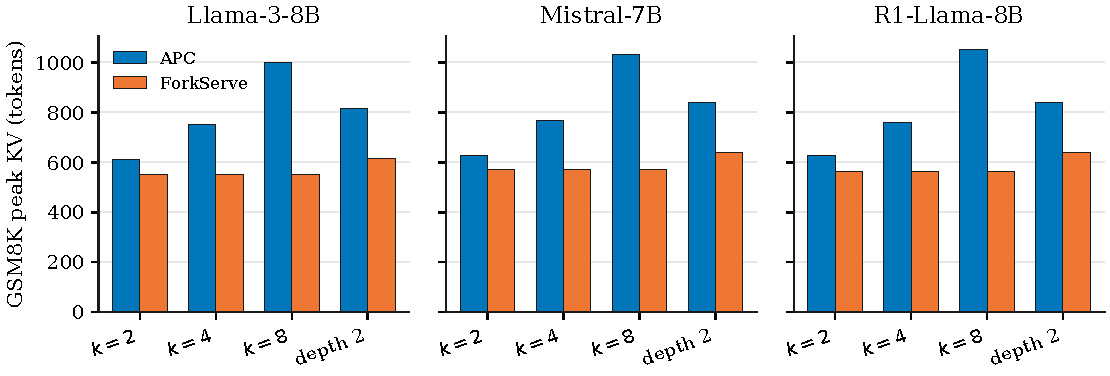
\includegraphics[width=\columnwidth]{fig/branch_peak.pdf}
\caption{\textbf{GSM8K peak KV versus branching} ($n{=}16$, $\mathrm{tp}{=}2$, $D{=}512$).
ForkServe+ matches the ForkServe bar.
The spine peak is invariant in $k$; the APC peak grows with the hashed union, so the ratio falls from $0.89$--$0.90$ to $0.53$--$0.55$.}
\label{fig:eval-branch}
\end{figure}

\paragraph{The ratio falls with $k$.}
\Cref{tab:branch,fig:eval-branch} measures $(L+\ell)/(L+k\ell)$ on the GPU. The spine peak is invariant in $k$ while the APC peak increases, so the ratio moves from $0.89$--$0.90$ at $k{=}2$ to $0.53$--$0.55$ at $k{=}8$ on all three families.
At depth $2$ the ratio is $0.75$--$0.76$.
ForkServe+ leaves the peak unchanged. At $k{=}8$ it rejects $28$ branches and reduces fan-out from $307$ to $179$\,ms on Llama-3-8B, from $349$ to $191$\,ms on Mistral-7B, and from $363$ to $194$\,ms on DeepSeek-R1.
With draft pruning disabled, Llama-3-8B fan-out is $247$\,ms and DeepSeek-R1 fan-out is $271$\,ms.
% The last-line stop is not the decode cut here: the winner already ends inside $D$, so emitted tokens stay near $2500$--$7000$ against APC's $8192$.
A batch of $16$ keeps the ratio at $0.72$--$0.73$ ($2071/2871$ on Llama-3-8B, $2135/2935$ on Mistral-7B, $2093/2893$ on DeepSeek-R1).

\begin{table}[t]
\centering
\caption{Contest forest, $D{=}2048$, $k{=}4$, $\mathrm{tp}{=}2$.
MATH-500 is $n{=}200$; AIME is $n{=}73$.
R1 is DeepSeek-R1; 4B is Qwen3-4B.
Best storage and shortest end-to-end time in green.}
\label{tab:longcot}
\scriptsize
\setlength{\tabcolsep}{2.4pt}
\setlength{\aboverulesep}{0.35pt}
\setlength{\belowrulesep}{0.35pt}
\begin{tabular}{llrrrr}
\rowcolor{tblhead}
\toprule
Model & Method & peak & / APC & acc. & e2e (s) \\
\midrule
 & APC & $1863$ & --- & $0.560$ & $429$ \\
\rowcolor{tblalt}
 & FS & \win{$1391$} & \win{$0.75$} & $0.510$ & $432$ \\
\multirow{-3}{*}{R1 MATH}
 & FS+ & $1599$ & $0.86$ & $0.545$ & \win{$247$} \\
\midrule
 & APC & $2118$ & --- & $0.055$ & $178$ \\
\rowcolor{tblalt}
 & FS & \win{$1646$} & \win{$0.78$} & $0.123$ & $178$ \\
\multirow{-3}{*}{R1 AIME}
 & FS+ & $1662$ & $0.78$ & $0.096$ & \win{$165$} \\
\midrule
 & APC & $1937$ & --- & $0.620$ & $329$ \\
\rowcolor{tblalt}
 & FS & \win{$1770$} & \win{$0.91$} & $0.625$ & $248$ \\
\multirow{-3}{*}{4B MATH}
 & FS+ & \win{$1770$} & \win{$0.91$} & $0.600$ & \win{$236$} \\
\midrule
 & APC & $2150$ & --- & $0.027$ & $136$ \\
\rowcolor{tblalt}
 & FS & \win{$1794$} & \win{$0.83$} & $0.041$ & $136$ \\
\multirow{-3}{*}{4B AIME}
 & FS+ & \win{$1794$} & \win{$0.83$} & $0.041$ & \win{$131$} \\
\bottomrule
\end{tabular}
\end{table}

At $D{=}2048$ the ratio is $0.75$--$0.91$ (\Cref{tab:longcot}).
On MATH-500, ForkServe matches APC ($432$\,s vs.\ $429$\,s on DeepSeek-R1).
ForkServe+ cuts DeepSeek-R1 from $429$\,s to $247$\,s and Qwen3-4B from $329$\,s to $236$\,s; the Qwen3-4B $n{=}32$ slice is $38$\,s versus $53$\,s.
ForkServe+ cuts MATH-500 fan-out from $2406$ to $1284$\,ms on DeepSeek-R1 and from $2787$ to $1014$\,ms on Qwen3-4B, against APC at $1593$ and $1201$\,ms.
Qwen3-4B ForkServe+ scores $120/200$ on MATH-500 (APC $124/200$).
